%!TEX root = ../dokumentation.tex

\chapter{Klassifikation anhand von Parteien} \label{ch:crispDm_1}

In dem folgenden Abschnitt wird \ac{CRISP-DM} genutzt, um \ac{ML} Modelle zu trainieren, welche Texte einer der sechs politischen Parteien aus dem Deutschen Bundestag zuordnet. 

% TODO: Add missing sections

\ac{CRISP-DM} ist ein weitverbreitetes iteratives Modell, welches zur Strukturierung von Data-Mining Projekten genutzt wird \autocite{martinez-plumed_casp-dm_2017, chapman_crisp-dm_2000}. Das Modell besteht aus sechs Schritten: Business Understanding, Data Understanding, Data Preparation, Modeling, Evaluation und Deployment. 

\begin{figure}[H]
    \centering
    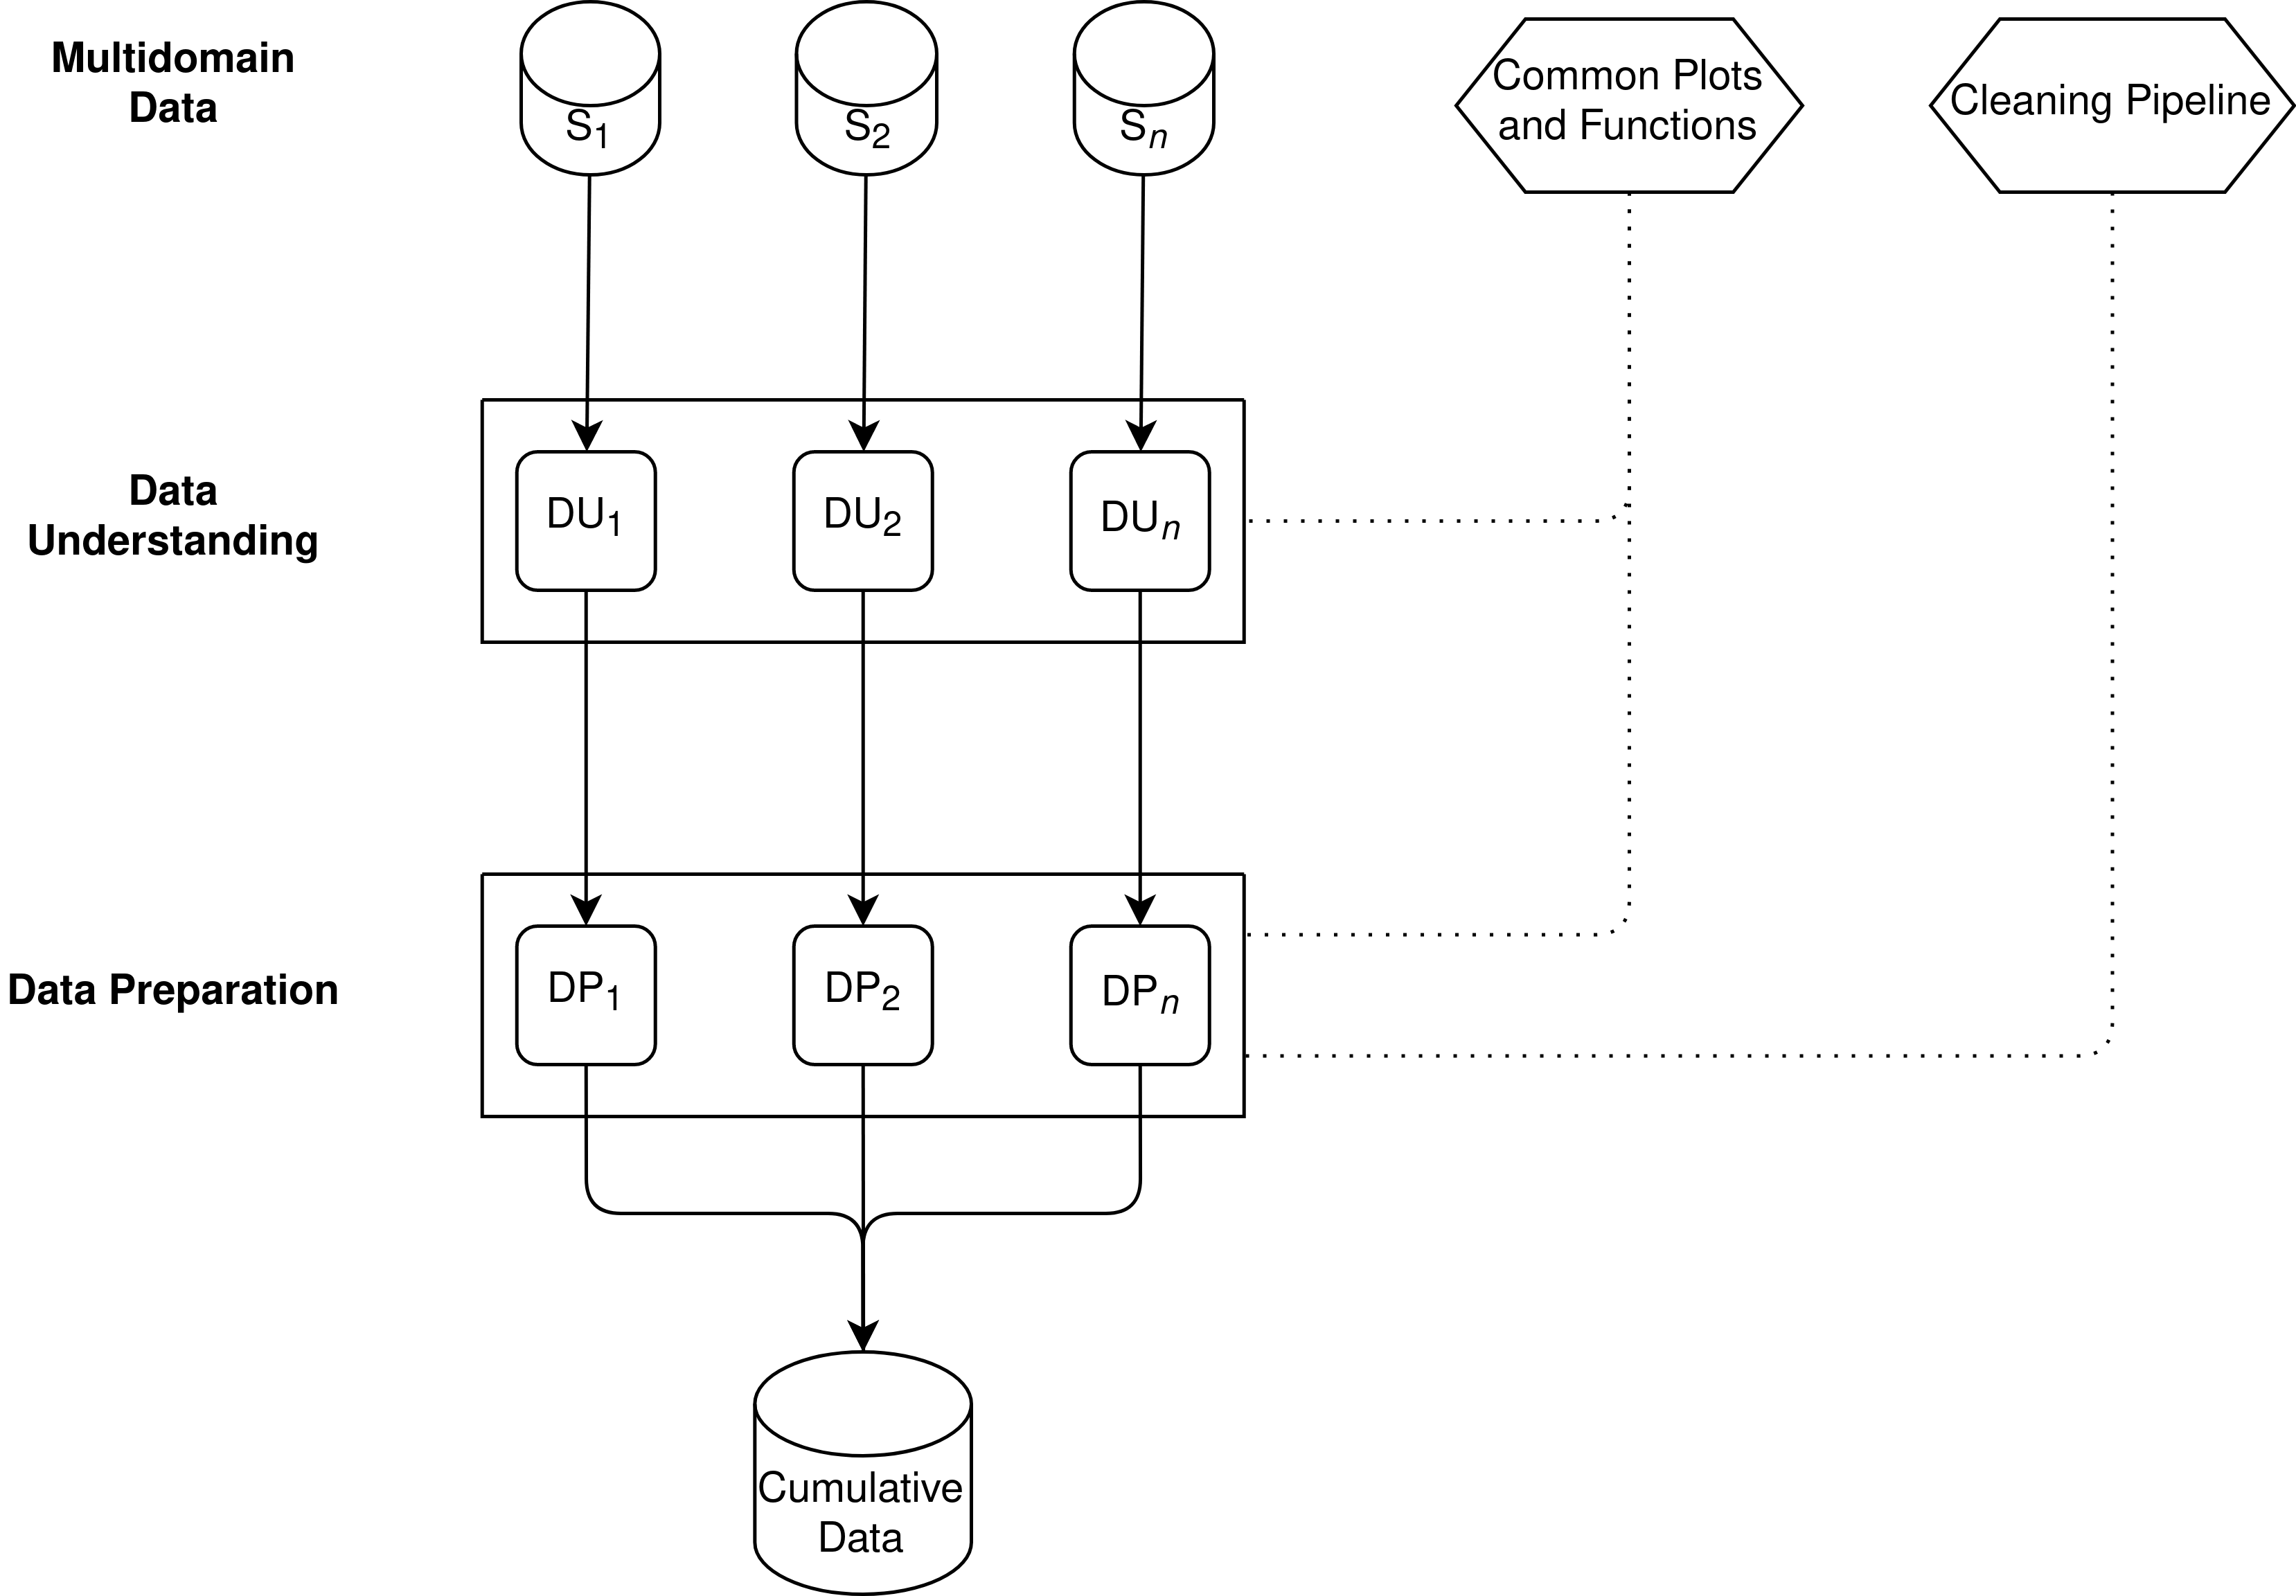
\includegraphics[width=0.8\textwidth]{data/images/data_flow_v2_1.png}
    \caption[Datenverarbeitungs-Pipeline]{Datenverarbeitungs-Pipeline (Data Understanding, Data Preparation und Zusammenführung der Daten)} \label{fig:dataFlow_1}
\end{figure}

% TODO: Add source for multidomain data

Multidomain Daten ermöglichen es, generalisierter \ac{ML} Modelle zu trainieren. Da die Rohdaten stark voneinander abweichen, ist es notwendig, dass unterschiedliche Datenquellen im Prozess des Data Understandings und Data Preparation individuell verarbeitet werden. Nachdem jeder Datensatz einzeln analysiert und bereinigt wurde, werden die Daten für das Modeling zusammengeführt.

% TODO: Update image for modeling

\begin{figure}[H]
    \centering
    \missingfigure{Data Flow 2}
    \caption[Training von Modellen]{Training von Modellen (Modeling)} \label{fig:dataFlow_2}
\end{figure}

\section{Sichtung der ausgewählten Datenquellen} \label{sec:dataUnderstanding}

Wie zuvor beschrieben, werden in dieser Arbeit verschiedene Datensätze genutzt, um die \ac{ML} Modelle zu trainieren. Damit soll vermieden werden, dass ein Modell lediglich die Eigenschaften eines spezifischen Datensatzes trainiert. 

Für das \nameref{sec:modeling} werden Datensätze benötigt, welche neben den Features (z. B. Text, Alter, Geschlecht) auch einer Partei zugeordnet sind. Da in dieser Form noch keine Datensätze vorhanden waren, wurden explizit Daten gewählt, welche von Politikern einer Partei veröffentlicht wurden. Somit kann die Parteizugehörigkeit als Zielvariable für das Training genutzt werden.

% TODO: Update values

\begin{table}[H]
    \centering
    {\footnotesize
    \begin{tblr}{width=\textwidth, hlines, vlines, colspec={Q[l,17mm]*{7}{Q[si={table-format=6},r]}}, row{1}={guard,font=\bfseries,l}, row{5}={font=\bfseries}}
        Datensatz & AfD & Die Grünen & SPD & Union & Die Linke & FDP & Gesamt\-anzahl \\ 

        Tweets\footnote{Tweets von den aufgeführten Parteien, exklusive parteilose Politiker} & 126132 & 167060 & 167647 & 157035 & 141738 & 112067 & 871679 \\
        Reden\footnote{Reden von den aufgeführten Parteien in dem Zeitraum der 19. Legislaturperiode.} & 4437 & 3857 & 5249 & 8007 & 3403 & 3888 & 28841 \\
        Wahlpro\-gramme & 2619 & 6399 & 4552 & 4564 & 5204 & 4376 & 27714 \\

        Summe & 133188 & 176861 & 177448 & 170246 & 150345 & 120331 & 928234 \\
    \end{tblr}
    }
    \caption{Anzahl an Einträgen pro Datensatz und pro Partei vor Bereinigen und Filtern} \label{tab:countPerDataset}
\end{table}

% TODO: Update num

Bei den Datensätzen handelt es sich um Tweets, Wahlprogramme (Landtags-, Europa- und Bundestagswahlen) und Reden aus dem Deutschen Bundestag. Wie aus \autoref{tab:countPerDataset} hervorgeht, umfassen die drei Datensätze initial \num{928234} Einträge. 

\subsection*{Tweets}

% TODO: Add source

Twitter ist eine amerikanische Kurznachrichten-Plattform, welche den Nutzern ermöglicht, Tweets\footnote{Plattformspezifische Bezeichnung für Kurznachrichten} von einer Länge von bis zu 280 Zeichen zu veröffentlichen. Zusätzlich zum Veröffentlichen von eigenen Tweets, besitzen Nutzer die Möglichkeit Tweets von anderen zu kommentieren, oder zu retweeten\footnote{Einen Tweet eines anderen Nutzers auf seinem eigenen Profil erneut veröffentlichen}.

Der Tweet-Datensatz\footnote{Aufgrund der Twitter Developer Bedingungen ist der Datensatz nicht öffentlich zugänglich. \citeauthor{saltzer_finding_2022} hat auf Anfrage den Datensatz für diese Arbeit zur Verfügung gestellt.} von \textcite{saltzer_finding_2022} umfasst \num{876118} Tweets von \num{511} Politikern des Deutschen Bundestages zwischen Januar \num{2017} bis Dezember \num{2019}. 

Der Datensatz beinhaltet neben den Tweet-Texten (\texttt{text}) auch noch den Twitternamen (\texttt{screen\_name}), das Erstellungsdatum (\texttt{created\_at}), ob es sich um einen Retweet handelt (\texttt{is\_retweet}), welcher Partei der Politiker angehört (\texttt{party}), das Geburtsdatum (\texttt{birthyear}) und das Geschlecht des Politikers (\texttt{gender}). Initial beinhaltet der Datensatz außerdem noch, ob der Politiker einer Untergruppierung einer Partei angehört und wie dieser bei Abstimmungen im Deutschen Bundestag abgestimmt hat. Diese letzten beiden Informationen werden jedoch im folgenden nicht weiter berücksichtigt.

Die Tweets der Parlamentarier lassen sich folgenden sechs Parteien\footnote{Initial beinhaltete der Datensatz zusätzlich Parteilose, welche jedoch direkt gefiltert wurden.} zuordnen: Die Grünen, \ac{SPD}, Die Linke, \ac{AfD}, \ac{FDP} und Union. Unter den \ac{MdB} befinden sich \num{161} Frauen und \num{350} Männer.

% TODO: Update image with correct image (pre-processing)

\begin{figure}[H]
    \centering
    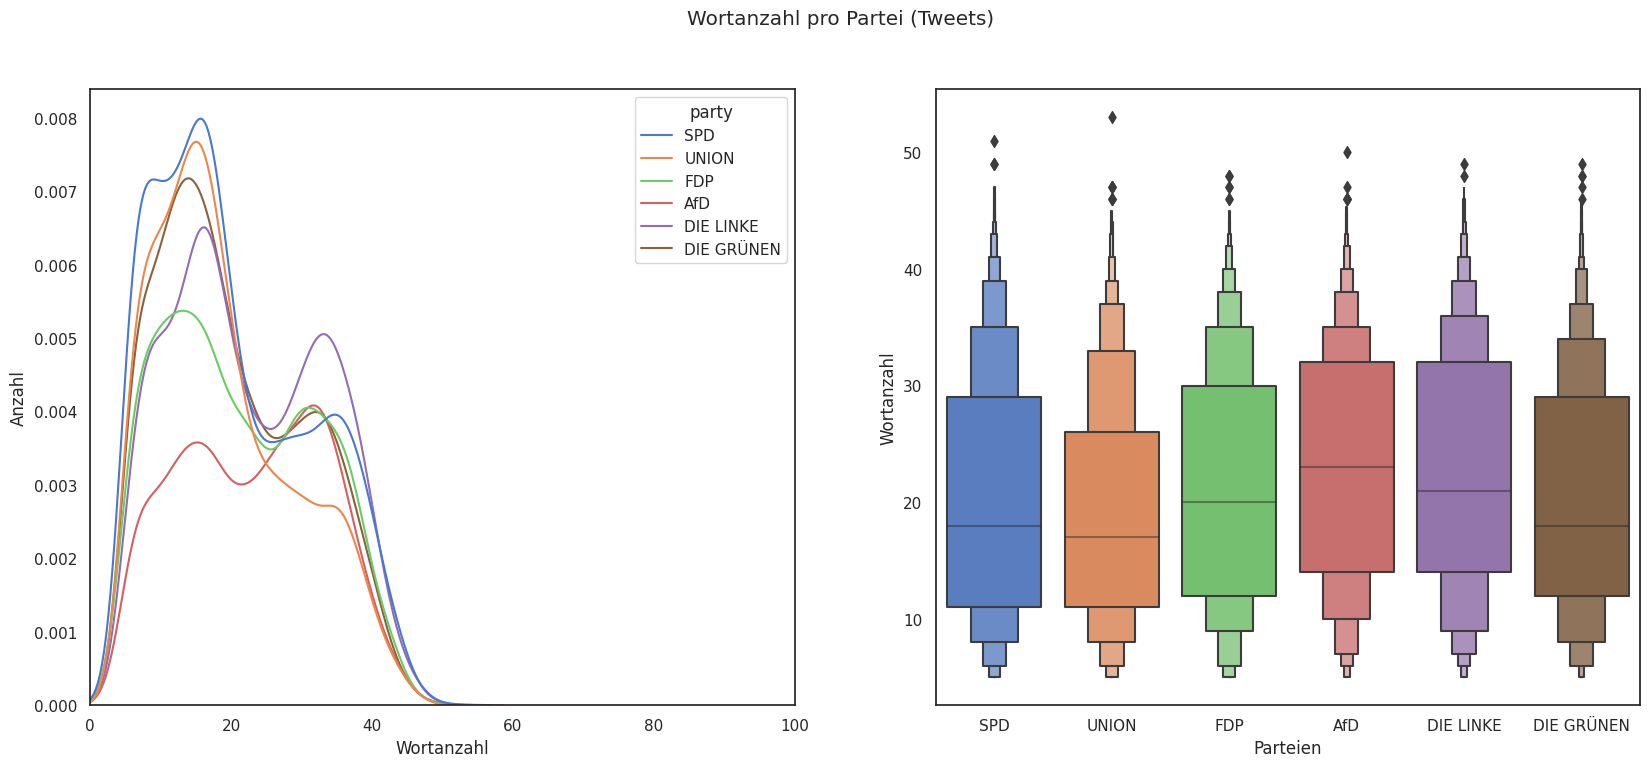
\includegraphics[width=0.9\textwidth]{data/images/tweets_word_count.png}
    \caption{Anzahl an Wörtern für Tweets vor Bereinigung} \label{fig:wordCountTweets}
\end{figure}

% TODO: Add reference

\autoref{fig:wordCountTweets} zeigt eine Dichtefunktion der Wortanzahl der Tweets gruppiert nach den einzelnen Parteien. Diese weisen jeweils zwei Extrema auf. Das Erste befindet sich im Bereich zwischen \num{15} bis \num{25} Wörtern und das Zweite im Bereich zwischen \num{30} bis \num{40} Wörtern. Im Durchschnitt veröffentlichen Politiker der Union vergleichsweise kurze Nachrichten, wohingegen die der \ac{AfD}, der \ac{FDP} und die der Linken vermehrt längere Nachrichten veröffentlichen.

\subsection*{Reden} \label{subsec:dataUnderstandingReden}

Als weitere Datenquelle sollen politische Reden, die von den Abgeordneten der verschiedenen Fraktionen im Bundestags gehalten worden sind, genutzt werden. Dabei kann auf den Datensatz \enquote{Open Discourse} von \textcite{richter_open_2021} zurückgegriffen werden, der alle Plenarprotokolle des Deutschen Bundestages von \num{1949} bis \num{2020} in Textform zur Verfügung stellt.

Neben den Reden, die im Folgenden als Trainingsdaten genutzt werden sollen, enthält der Datensatz auch alle Zwischenrufe und -fragen, die von Parlamentariern während der Debatten geäußert wurden. Aufgrund von mangelnder Qualität und Länge dieser werden sie für den weiteren Verlauf der Arbeit als Datenquelle verworfen.

Zusätzlich zum Text (\texttt{speechContent}) liegen für jede Rede unter anderem zusätzlich die Nummer der Sitzung des Bundestages (\texttt{session}), das Datum (\texttt{date}), Vor- und Nachname (\texttt{firstName} bzw. \texttt{lastName}), die Fraktion (\texttt{factionId}) sowie die Position des Redners (\texttt{positionLong}) vor.

Über alle Wahlperioden hinweg enthält der Datensatz insgesamt \num{907644} Reden von \num{4105} Politikern. Da sich das zu trainierende Klassifikationsmodell im Rahmen dieser Arbeit nur auf die 19. Wahlperiode bezieht, werden nur Reden berücksichtigt, die auch in dem genannten Zeitraum gehalten wurden, wodurch noch \num{60958} Reden übrig bleiben. Die übrigen Reden umfassen jedoch auch Beiträge des Präsidiums des Deutschen Bundestages sowie fraktionsloser Abgeordneter, die beide nicht betrachtet werden können, da sie keiner der definierten Parteien zuzuordnen sind. Somit reduziert sich die Zahl an Reden schlussendlich auf \num{28841}.

% TODO: Verteilung der Reden nach Partei

\begin{figure}[H]
    \centering
    \includegraphics[width=0.9\textwidth]{data/images/speeches_word_count.png}
    \caption{Anzahl an Wörtern für Reden vor Bereinigung} \label{fig:wordCoundSpeeches}
\end{figure}

\autoref{fig:wordCoundSpeeches} zeigt die Verteilung der Anzahl an Wörtern, die die Reden im Datensatz umfassen, aufgeschlüsselt nach Partei. Es ergibt sich dabei ein Hochpunkt in der Dichtefunktion bei knapp unter 100 Wörtern, gefolgt von einem Tiefpunkt zwischen \num{200} und \num{300} Wörtern und schließlich einem weiteren Hochpunkt, je nach Partei zwischen 400 und 700 Wörtern.

Dies zeigt, dass die Reden im Durchschnitt etwa um den Faktor zehn länger sind als Tweets, was darauf zurückzuführen ist, dass die Reden im Bundestag oft mehrere Minuten andauern, während Tweets als Kurznachrichten gedacht sind.

Bei genauerer Betrachtung der Häufung von kurzen Reden rund um das erste Maximum fällt auf, dass dort viele Redebeiträge enthalten sind, die nur beispielsweise Zwischenfragen darstellen und keine vollständigen, inhaltlich relevanten Reden sind.

% TODO: Beispiele für kurze Reden / Zwischenfragen im Anhang

\subsection*{Wahlprogramme}

Zuletzt sollen auch Texte aus Wahlprogrammen der zu untersuchenden Parteien herangezogen werden. Dabei stehen im Untersuchungszeitraum die Bundestagswahlen \num{2017} und \num{2021}, die Europawahl 2019 sowie zahlreiche Landtagswahlen mit den entsprechend veröffentlichten Wahlprogrammen der Parteien zur Verfügung. Eine genaue Auflistung der verwendeten Wahlen inklusive Anmerkungen zu Wahlprogrammen, die nicht verarbeitet werden konnten, kann dem \autoref{subsec:übersichtWP} im Anhang entnommen werden.

So ergibt sich eine Anzahl von insgesamt \num{83} Wahlprogrammen unterschiedlicher Parteien. Die Wahlprogramme können auf der Website der jeweiligen Partei bzw. des Landesverbandes im Fall einer Landtagswahl im \ac{PDF}-Format heruntergeladen werden. Anschließend wird der Text mittels der Python-Bibliothek \textit{pdfminer} ausgelesen und verarbeitet.

Damit aus den Wahlprogrammen kohärente, kürzere Texte extrahiert werden können, wird jedes Wahlprogramm nach Absätzen unterteilt, sodass sich eine Gesamtanzahl von \num{28783} Paragraphen als Trainingsdaten vor der Bereinigung ergibt.

Neben dem Text des jeweiligen Paragraphen liegen als weitere Informationen, die während des Auslesens der Wahlprogramme gesammelt wurden, die Partei, aus deren Wahlprogramm der Text entnommen wurde (\texttt{party}), die Art der Wahl (\texttt{election\_type})\footnote{Bundestags-, Europa- oder Landtagswahl} und ein Kürzel für die Wahl (\texttt{election})\footnote{Bestehend aus Art der Wahl, gegebenenfalls Bundesland und Jahr} vor.

\begin{figure}[H]
    \centering
    \includegraphics[width=0.9\textwidth]{data/images/party_programs_word_count.png}
    \caption{Anzahl an Wörtern für Wahlprogramm-Paragraphen vor Bereinigung} \label{fig:wordCoundPartyPrograms}
\end{figure}

\autoref{fig:wordCoundPartyPrograms} zeigt die Verteilung der Anzahl an Wörtern der gewonnenen Wahlprogramm-Paragraphen pro Partei. Anders als bei den Reden zeigt sich hier eine rechtsschiefe Dichtefunktion mit nur einem Maximum bei -- je nach Partei -- etwa \num{30} bis \num{70} Wörtern pro Paragraph. Damit sind die Absätze aus Wahlprogrammen durchschnittlich länger als die Tweets, jedoch deutlich kürzer als die Transkripte der Bundestagsreden. 


\section{Datenaufbereitung} \label{sec:dataPreparation}

Im nächsten Schritt nach \ac{CRISP-DM} werden die Datensätze aufbereitet. Im Folgenden werden zwei Methoden verwendet, um dies zu erreichen. Zum Ersten, Techniken, die die Integrität der Texte verändert. Dies umfasst regelbasierte Verfahren, die Bildung von Wortstämmen und das Entfernen von Stopwörtern. Anschließend werden Eigenschaften definiert, nach welchen die Texte gefiltert werden. Hierbei wird die Integrität der Text nicht weiter beeinflusst.

\subsection{Datenbereinigungs-Pipeline} \label{subsec:cleaningPipeline}

Stopwörter, Links, Symbole und weitere Unregelmäßigkeiten (Rauschen, zu Englisch \textit{Noise}) beeinflussen die Performance von \ac{ML} Modellen stark \autocite[4]{kowsari_text_2019}. Daher ist es notwendig Texte mittels regelbasierten Verfahren, als auch mit \ac{ML} Verfahren zu bereinigen. 

% TODO: Add more details for "Regelbasiertes Bereinigen" and add tokenizing to lemmatizing

\begin{figure}[H]
    \centering
    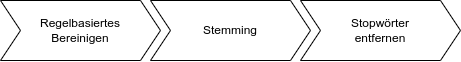
\includegraphics[width=0.7\linewidth]{data/images/cleaning_pipeline_v1.png}
    \caption{Datenbereinigungsprozess} \label{fig:cleaningPipeline}
\end{figure}

Wie \autoref{fig:cleaningPipeline} zeigt, besteht der Prozess zur Datenbereinigung aus drei Abschnitten. Zuerst die regelbasierte Bereinigung, welche mittels regulären Ausdrücken und Patterns eine erste Umformung vornimmt. Im nächsten Schritt werden die Wörter auf ihren Wortstamm zurückgeführt. Im letzten Schritt werden Stopwörter entfernt. All diese Schritte verfolgen das Ziel, die Menge an Rauschen zu verringern. 

\subsubsection{Regelbasierte Verfahren}

Unterschiedliche Schreibweisen, Symbole und Emojis, \acp{URL}, und Gendern stellen ein elementares Problem für herkömmliche \ac{NLP} Methoden und Modelle dar \autocite[4\psq]{kowsari_text_2019}. Im ersten Schritt werden daher regelbasierte Verfahren genutzt, um häufig auftretende Zeichen, Symbole/Emojis, aber auch andere Unregelmäßigkeiten ersetzt oder entfernt.

Besonders bei Tweets werden häufig Symbole wie \euro und \& als Kurzform verwendet. Da diese jedoch nicht in dieser Form interpretiert werden können, werden die Symbole als auch die Zahlen mit ihrem ausgeschriebenen Klartext ersetzt. So wird aus \euro \(\rightarrow\) \textit{euro}, oder aus \(\num{2000} \rightarrow\) \textit{zweitausend}.

In den Texten treten vermehrt Unicode, \ac{HTML} Symbole, als auch Emojis auf. In Tweets als auch in Wahlprogrammen werden ebenfalls \acp{URL} verwendet. Tweets nutzen außerdem Referenzen zu Twitternutzern (Mentions wie \textit{@MaxMustermann}). Da es sich bei all diesen Symbolgruppen um nicht vollständige oder nicht interpretierbare Zeichenketten handelt, müssen diese entfernt werden.

Bei allen Textformen verwenden Politiker und Parteien unterschiedliche Arten von inklusiver Sprache als Alternative zum generischen Maskulinum. Beispiele hierfür sind \textit{Politiker*innen} oder auch \textit{Politiker:innen}. Da die Textrepräsentationsformen und Sprachmodelle dies jedoch nur rudimentär oder gar nicht abbilden können, werden alle herkömmlichen Endungen für gendergerechte Sprache entfernt, sodass alle Wörter im Text auf den korrekten Wortstamm reduziert werden können.

Nachdem die Texte grob bereinigt wurden, werden letztlich noch Satzzeichen, Sonderzeichen und einzelne Buchstaben entfernt. Abschließend werden doppelte Leerzeichen entfernt und alle Buchstaben zu Kleinbuchstaben umgewandelt.

% TODO: Update tweet example

\begin{code}[H]
    \begin{subcode}{0.45\textwidth}
        \small
        \textcolor{orange}{Ehemalige} \textcolor{red}{@AfD-Vorsitzende} \textcolor{orange}{\#Petry} muss wegen \textcolor{orange}{Meineid} vor \textcolor{orange}{Gericht}\textcolor{red}{.} \textcolor{orange}{Kein Einzelfall}\textcolor{red}{:} gegen circa \textcolor{orange}{\SI{10}{\percent}} aller \textcolor{orange}{AfD-Abgeordneten} bundesweit laufen oder liefen \textcolor{orange}{Strafverfahren}\textcolor{red}{.} \textcolor{orange}{Kriminelle Asylbewerber}\textcolor{red}{?} \textcolor{orange}{Fehlanzeige}\textcolor{red}{.} \textcolor{orange}{Kriminelle AfD-Hetzer} trifft den \textcolor{orange}{Nagel} eher auf den \textcolor{orange}{Kopf} \textcolor{red}{<U+0001F602>} \textcolor{orange}{\#AfD}
        \caption{Tweet vor jeglicher Bereinigung}
    \end{subcode}\hfill
    \begin{subcode}{0.45\textwidth}
        \small
        ehemalige petry muss wegen meineid vor gericht kein einzelfall gegen circa zehn prozent aller afd abgeordneten bundesweit laufen oder liefen strafverfahren kriminelle asylbewerber fehlanzeige kriminelle afd hetzer trifft den nagel eher auf den kopf afd
        \caption{Tweet nach regelbasierter Bereinigung}
    \end{subcode}\hfill
    \caption[Beispiel -- Regelbasierte Bereinigung]{Beispiel für regelbasierte Bereinigung eines Tweets von \textit{victorperli}} \label{list:rulebasedCleaning}
\end{code}

\autoref{list:rulebasedCleaning} zeigt die Anwendung der regelbasierten Bereinigung auf einen Beispiel-Tweet. Es kann erkannt werden, dass die Referenz \textit{@AfD-Vorsitzende} im bereinigten Text nicht mehr vorkommt. Zudem wurde das Hashtag-Symbol vor \textit{Petry} und \textit{AfD} entfernt. Auch die Angabe \textit{10\%} wird durch die Bereinigung ausgeschrieben zu \textit{zehn prozent}. Schließlich enthält der bereinigte Text auf der rechten Seite keine Satzzeichen mehr, das Emoji am Ende fehlt und alle Wörter sind kleingeschrieben, sodass nur noch korrekte Wörter vorkommen.

Bei den Redetexten ist zusätzlich zu beachten, dass im Datensatz Zwischenrufe von anderen Politikern im Redetext durch Referenzen -- gekennzeichnet durch eine Zahl innerhalb geschweifter und normaler Klammern -- vorkommen. Da der Text nur den Inhalt der Rede selbst beinhalten soll, werden die Referenzen zu den Zwischenrufen mithilfe eines regulären Ausdrucks entfernt.

Bei dem Auslesen der Wahlprogramme werden die Paragraphen nach Leerzeilen getrennt, wobei manche Absätze allerdings über das Seitenende hinaus weitergehen. Daher werden Paragraphen, die nicht mit einem Satzzeichen enden, mit darauffolgenden Paragraphen zusammengefügt. Zudem kommt es bei einigen Dokumenten dazu, dass Text aus der Kopf- und Fußzeile sowie von Anmerkungen an der Seite des regulären Textes mit ausgelesen wird. Da dieser folglich ungewollt in den übrigen Abschnitten enthalten ist, muss er im Rahmen der regelbasierten Bereinigung auch entfernt werden.

\subsubsection{Wortstamm}

Der nächste Schritt dient dazu, die Wörter zu vereinheitlichen. Hierfür werden Wörter mit dem dazugehörigen Wortstamm ersetzt (\textit{eng. Lemmatizing}). Für die Umwandelung wurde \href{https://spacy.io/}{\texttt{spacy}} verwendet

% TODO: Update tweet example

\begin{code}[H]
    \begin{subcode}{0.45\textwidth}
        \small
        \textcolor{orange}{ehemalige} petry muss wegen meineid vor gericht kein einzelfall gegen circa zehn prozent aller afd \textcolor{orange}{abgeordneten} bundesweit laufen oder liefen \textcolor{orange}{strafverfahren} \textcolor{orange}{kriminelle} asylbewerber \textcolor{orange}{fehlanzeige} \textcolor{orange}{kriminelle} afd hetzer \textcolor{orange}{trifft} \textcolor{orange}{den} nagel eher auf den kopf afd
        \caption{Tweet nach regelbasierter Bereinigung}
    \end{subcode}\hfill
    \begin{subcode}{0.45\textwidth}
        \small
        ehemalig petry muss wegen meineid vor gericht kein einzelfall gegen circa zehn prozent aller afd abgeordneter bundesweit laufen oder laufen strafverfahr kriminell asylbewerber fehlanzeig kriminell afd hetzer treffen der nagel eher auf der kopf afd
        \caption{Tweet nach dem Bilden der Wortstämme}
    \end{subcode}\hfill
    \caption[Bildung von Wortstämmen]{Beispiel für die Bildung von Wortstämmen eines Tweets von \textit{victorperli}} \label{list:lemma}
\end{code}

Wie in \autoref{list:lemma} zu erkennen, werden unter anderem Endungen wie \textit{e} und \textit{en} mit dem jeweiligen Stamm ersetzt. Wenn Wörter nicht in dem Wörterbuch enthalten sind, werden diese exkludiert.

\subsubsection{Stopwörter}

% TODO: Add more sources

Stopwörter sind Füllwörter, welche keine starke Relevanz für die Bedeutung eines Satzes haben \autocite[4]{kowsari_text_2019}. Das dadurch entstehende Rauschen kann unterdrückt werden, indem die Stopwörter gefiltert werden.

% TODO: Update tweet example

\begin{code}[H]
    \begin{subcode}{0.45\textwidth}
        \small
        ehemalig petry \textcolor{red}{muss wegen} meineid \textcolor{red}{vor} gericht \textcolor{red}{kein} einzelfall \textcolor{red}{gegen} circa zehn prozent \textcolor{red}{aller} afd abgeordneter bundesweit laufen \textcolor{red}{oder} laufen strafverfahr kriminell asylbewerber fehlanzeig kriminell afd hetzer treffen \textcolor{red}{der} nagel eher \textcolor{red}{auf der} kopf afd
        \caption{Tweet nach dem Bilden der Wortstämme}
    \end{subcode}\hfill
    \begin{subcode}{0.45\textwidth}
        \small
        ehemalig petry wegen meineid gericht einzelfall circa zehn prozent afd abgeordneter bundesweit laufen laufen strafverfahr kriminell asylbewerber fehlanzeig kriminell afd hetzer treffen nagel eher kopf afd
        \caption{Tweet nach dem Entfernen von Stopwörtern}
    \end{subcode}\hfill
    \caption[Beispiel -- Entfernen von Stopwörtern]{Beispiel für das Entfernen von Stopwörtern eines Tweets von \textit{victorperli}} \label{list:stopwords}
\end{code}

Für das Filtern, wie in \autoref{list:stopwords} gezeigt, wurde das Stopwort-Lexikon von \href{https://www.nltk.org/}{\texttt{nltk}} für die deutsche Sprache verwendet. Wie das Beispiel zeigt, werden häufig auftretende Wörter ohne stärkeren Kontext und ohne Bedeutung für den zentralen Sinn für den Text entfernt.

\subsection{Filtering} \label{subsec:filtering}

Auf Basis der Erkenntnisse aus \nameref{sec:dataUnderstanding} werden im Folgenden die Datensätze gefiltert. Dies ist wichtig, um die Datenqualität zu erhöhen und etwaige Bias zu vermeiden.

\subsubsection*{Tweets} \label{subsubsec:filteringTweets}

% TODO: Add wordcloud

Der Tweet-Datensatz \textcite{saltzer_finding_2022} weist Tweet-Duplikate auf. Diese sind jeweils von dem gleichen Politiker verfasst und weisen den gleichen Text auf. Lediglich das Erstellungsdatum (\texttt{created\_at}) des Eintrages weicht bei den Duplikaten voneinander ab. Da dies auf einen Fehler beim Data-Mining hindeutet, werden lediglich die neusten Einträge dieser Duplikate behalten.

Des Weiteren existieren Einträge, bei denen der Tweet-Text als auch das \texttt{is\_retweet} Label, leer ist. Da beide dieser Datenpunkte benötigt werden, werden diese Einträge ebenfalls komplett entfernt. 

Tweets, welche lediglich von Politikern retweetet werden, lassen sich nicht eindeutig dem Politiker selbst und seinen Ansichten zuordnen. Es könnte also sein, dass ein Politiker einen Tweet entweder retweetet, weil er der Aussage und Meinung zustimmt, oder auch falls er komplett andere Ansichten hat und seine Reichweite nutzen möchte, um Aufmerksamkeit auf den Autor und das Thema zu lenken. Aufgrund dieser Ungewissheit werden Tweets, welche als Retweet gegengezeichnet werden, entfernt.

Wie schon mittels \autoref{fig:wordCountTweets} festgestellt, werden vermehrt kurze Tweets (\num{15} bis \num{25}) und lange Tweets (\num{30} bis \num{40}) veröffentlicht. Bei Tweets mit weniger als \num{10} Wörtern ist es schwierig, einen tieferen Kontext festzustellen. Daher werden diese Tweets, entfernt (\texttt{stemm\_text >= 10}).

\subsubsection*{Reden}

Wie in \autoref{subsec:dataUnderstandingReden} erläutert, enthält der Datensatz bestehend aus politischen Reden von \citeauthor{richter_open_2021} nicht nur Reden zur 19. Wahlperiode des Deutschen Bundestages, sondern auch ältere. Daher muss der Datensatz in einem ersten Schritt auf den entsprechenden Untersuchungszeitraum begrenzt werden.

Ferner können als Trainingsdaten für das Klassifikationsmodell nur Texte verwendet werden, die einer der sechs Fraktionen im Bundestag zuzuordnen sind. Daher müssen auch Redebeiträge von fraktionslosen Abgeordneten sowie des Präsidiums ausgeschlossen werden.

Bei der Betrachtung der Anzahl an Wörtern in Reden (siehe \autoref{subsec:dataUnderstandingReden}) ist aufgefallen, dass es eine Häufung von vergleichsweise kurzen Texten mit einer Länge von unter \num{200} Wörtern gibt. Da bei diesen nicht sichergestellt werden kann, dass sie ausreichend politischen Inhalt bieten, als auch der Kontext der Aussagen klar wird, werden im weiteren Verlauf nur noch Reden mit mindestens 200 Wörtern berücksichtigt (\texttt{word\_count >= 200}).

Damit die Texte ohne Probleme von vortrainierten Sprachmodellen als Eingabe genutzt werden können, ist es erforderlich, lange Reden in mehrere kleinere Textabschnitte aufzuteilen, da sonst die maximale Anzahl an Eingabe-Tokens\footnote{Bei BERT-basierten Modellen, die für das Modeling genutzt werden sollen, sind es maximal 512 Tokens.} überschritten werden würde. Dabei wird darauf geachtet, dass eine Rede nur nach einem abgeschlossenen Satz aufgetrennt wird, um die Qualität der Daten nicht zu verringern.

Der Datensatz enthält außerdem drei Einträge mit dupliziertem Text, die daher ausgeschlossen werden.

\subsubsection*{Wahlprogramme}
Da die Daten zu den Wahlprogrammen selbst gesammelt und verarbeitet wurden, gibt es keine Einträge aus einem falschen Zeitraum oder von einer nicht zu untersuchenden Partei.

Bereits im Zuge des Auslesens der \ac{PDF}-Dateien der Wahlprogramme wurden nur Absätze mit mindestens \num{150} Zeichen weiterverarbeitet, da es sich ansonsten mehrheitlich um kurze Überschriften handelt. Da die Abschnitte im Vergleich zu den Reden deutlich kürzer sind, ist keine Obergrenze für die Länge nötig, um die weitere korrekte Verarbeitung zu garantieren.

Auch bei den Wahlprogramm-Texten lassen sich einige Duplikate finden, die herausgefiltert werden müssen.


\section{Aufbereitete Datensätze} \label{sec:processedDataframes}

Nach Anwendung der Datenbereinigungs-Pipeline bleiben im Gesamt-Datensatz etwa \num{395000} Einträge übrig. Damit hat sich die Größe des Datensatzes stark reduziert, vor allem viele ursprüngliche Tweet-Daten sind nicht mehr enhalten. \autoref{tab:countPerDatasetAfterCleaning} zeigt die Anzahl an Einträgen in den drei Datensätzen sowie pro Partei.

% TODO: Add correct nums
\begin{table}[H]
    \centering
    {\footnotesize
    \begin{tblr}{width=\textwidth, hlines, vlines, colspec={l*{7}{Q[si={table-format=5},r]}}, row{1}={guard,font=\bfseries,l}, row{5}={font=\bfseries}}
        Datensatz & AfD & Die Grünen & SPD & Union & Die Linke & FDP & Gesamt\-anzahl \\ 

        Tweets & 39840 & 60390 & 62227 & 54391 & 59473 & 50304 & 326625 \\
        Reden & 5750 & 4745 & 8015 & 12209 & 4558 & 4983 & 40260 \\
        Wahlpro\-gramme & 2618 & 6398 & 4552 & 4560 & 5203 & 4343 & 27674 \\

        Summe & 48208 & 71533 & 74794 & 71160 & 69234 & 59630 & 394559 \\
    \end{tblr}
    }
    \caption{Anzahl an Einträgen pro Datensatz und pro Partei nach Bereinigen und Filtern} \label{tab:countPerDatasetAfterCleaning}
\end{table}

Im Folgenden werden die Texte und weitere Features der Tweets, Reden und Wahlprogramme genauer untersucht. Im Gegensatz zum Stand vor der Bereinigung ist es an dieser Stelle möglich, die Texte ohne signifikante Beeinflussung durch nicht verarbeitbaren Zeichen oder falsche Einträge zu analysieren, um erste Erkenntnisse und Unterschiede zwischen den Parteien zu identifizieren.

% \begin{itemize}
    % \item Nach dem Cleaning lassen sich starke Veränderungen in der Anzahl an Wörtern bei den einzelnen Parteien feststellen. Zum Beispiel waren die Tweets der \ac{FDP} im Schnitt am längsten, was nach der Bereinigung nicht mehr der Fall ist. Das bedeutet, dass die \ac{FDP} entweder überdurchschnittlich viele Links und Markierungen anderer Nutzer oder deutlich mehr Füllwörter als andere Parteien verwendet.
    % \item Anzahl an Politikern/Beiträge pro Partei
    % \item Durchschnittliche Anzahl an Tweets pro Politiker pro Partei
    % \item Wordcloud mit häufigsten Wörtern
    % \item Häufigste n-grams
    % \item Timeplot Anzahl and Tweets pro monat
    % \item Stentiment Analysis Ergebnis
    % \item Wortanzahl nach Bereinigung
    % \item Geschlechtverteilung pro Partei
% \end{itemize}

\subsection*{Tweets}

Aus \autoref{tab:countPerDatasetAfterCleaning} geht hervor, dass sich die Anzahl an Tweets nach dem Filtern um \SI{62.53}{\percent} reduziert hat. Wie in \autoref{subsubsec:filteringTweets} beschrieben, wurden Duplikate, Retweets und zu kurze Tweets entfernt.

% TODO: Update figure
% TODO: Plot before cleaning to check behavior

\begin{figure}[H]
    \centering
    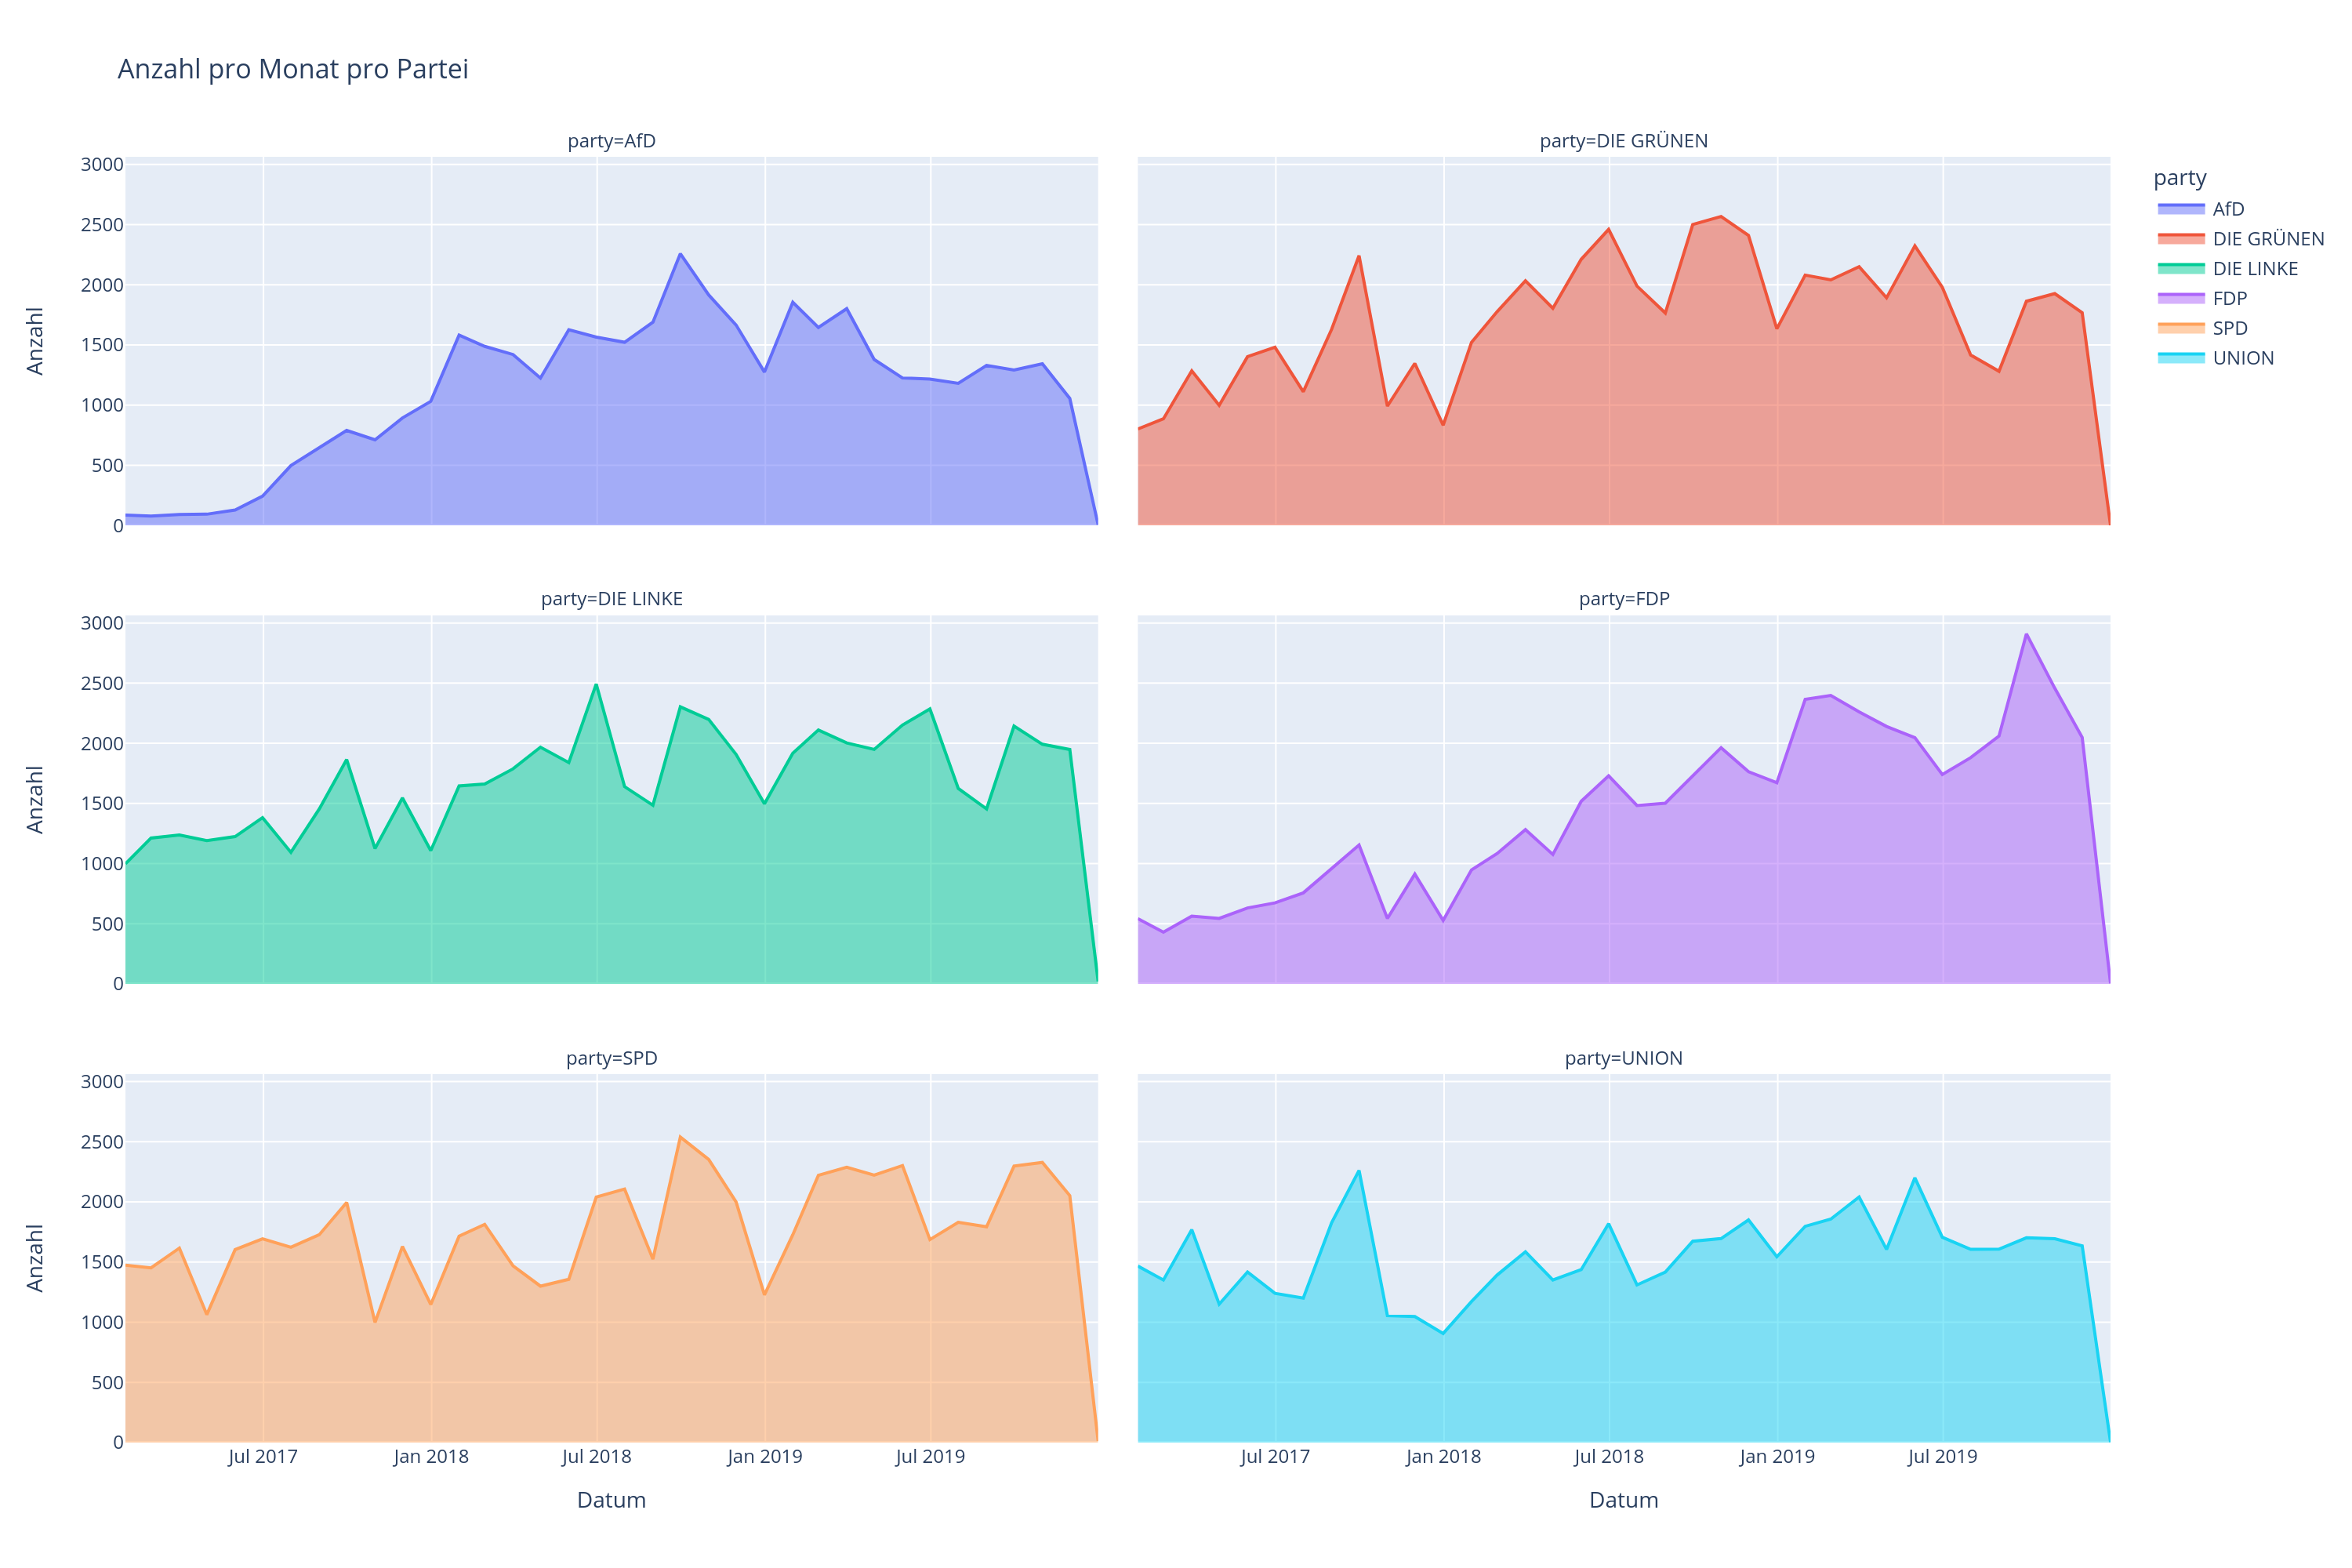
\includegraphics[width=\linewidth]{data/images/anzahl_pro_monat_pro_partei.png}
    \caption{Anzahl an Tweets pro Monat nach Partei} \label{fig:countTweetsTimeline}
\end{figure}

Wie aus \autoref{fig:countTweetsTimeline} zu erkennen, weisen besonders zwei Parteien starke Auffälligkeiten auf. Zum einen die \ac{AfD}, bei der besonders am Anfang des Zeitraums verhältnismäßig wenige Tweets gesammelt wurden. Weiterhin ist ebenfalls der Verlauf der \ac{FDP} auffällig. Diese weist einen starken Zuwachs in der Anzahl an Tweets über den gesammelten Zeitraum auf. Bei den Grünen lässt sich eine leichte Zunahme in der Anzahl in der Mitte des Zeitraums feststellen. Die Linke, \ac{SPD} und Union sind nicht weiter auffällig, mit der Ausnahme von einzelnen lokalen Extrema.

% TODO: Check wether to round 2 or 4

\begin{table}[H]
    \centering
    {\footnotesize
    \begin{tblr}{width=\textwidth, hlines, vlines, colspec={l*{3}{Q[si={table-format=1.2},c]}}, row{1}={guard,font=\bfseries,l}} 
        Partei & Negative & Neutral & Positive \\
        
        AfD & 0.28 & 0.68 & 0.04 \\
        DIE GRÜNEN & 0.20 & 0.74 & 0.06 \\
        DIE LINKE & 0.21 & 0.75 & 0.04 \\
        FDP & 0.22 & 0.73 & 0.05 \\
        SPD & 0.18 & 0.74 & 0.09 \\
        UNION & 0.16 & 0.78 & 0.07 \\
    \end{tblr}
    }
    \caption{Prozentuale Sentimentverteilung} \label{tab:sentimentDistributionTweet}
\end{table}

Auffällig bei den Tweets ist, dass besonders die Regierungsparteien -- Union und \ac{SPD} -- sich weniger negativ äußern als die Oppositionsparteien. Bei den positiven Tweets zeigt sich ein invertiertes Verhalten, wobei allgemein die Rate an positiven Tweets deutlich geringer ist.

\begin{figure}[H]
    \centering
    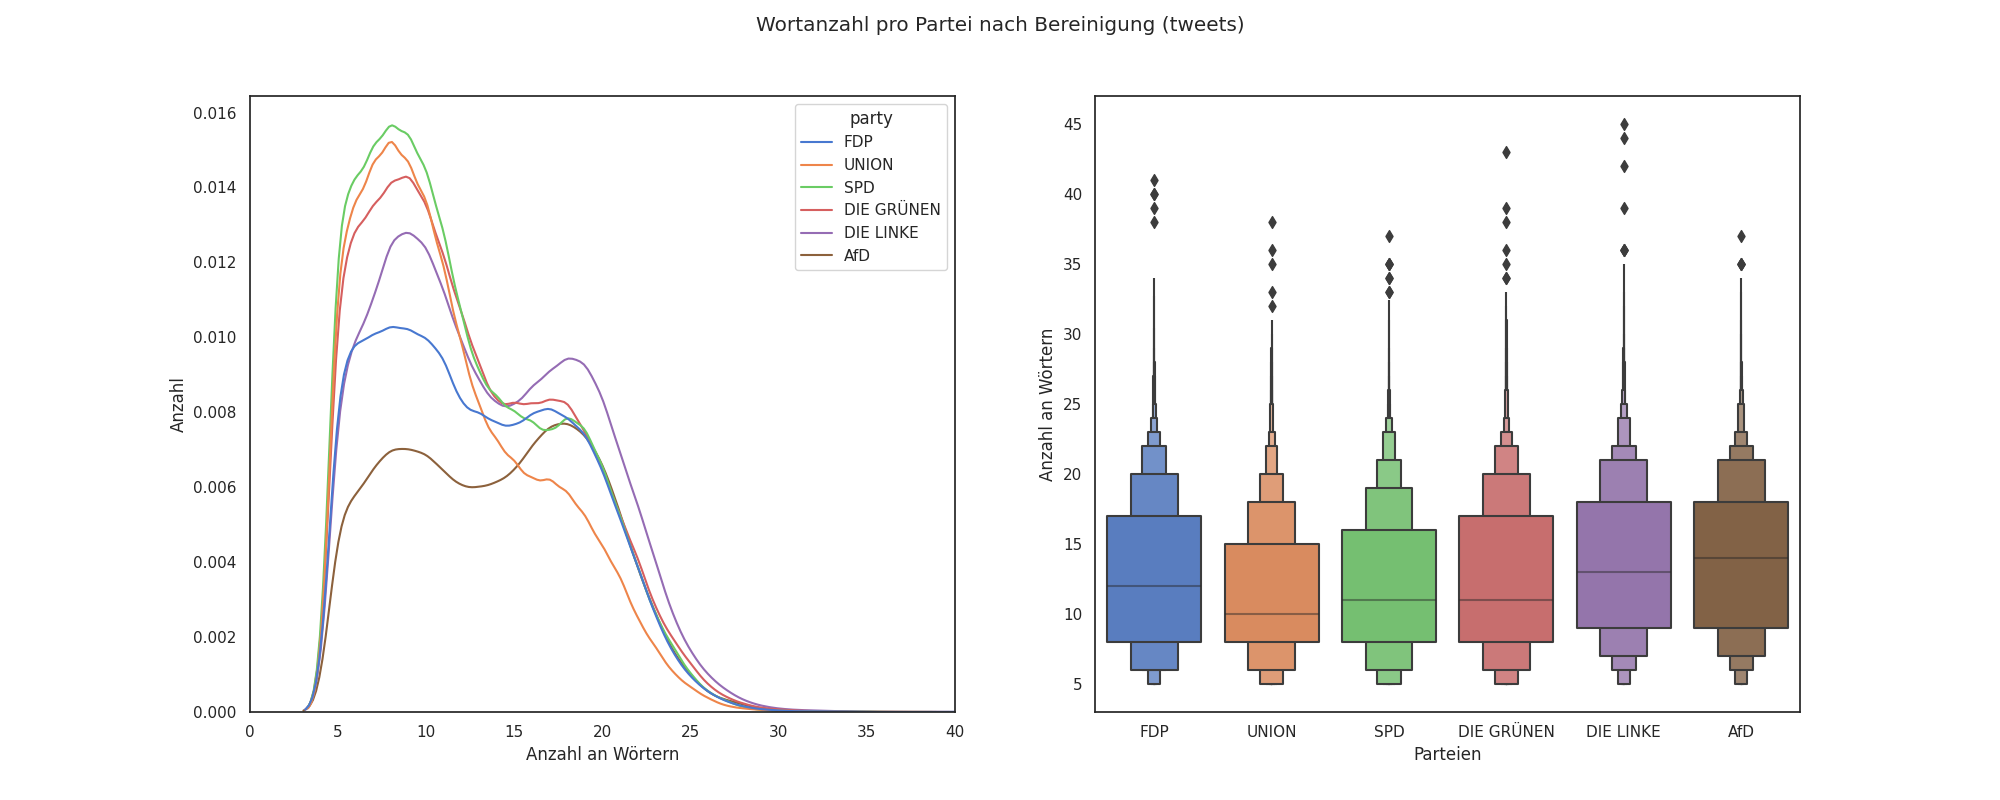
\includegraphics[width=\linewidth]{data/images/wortanzahl_pro_partei_nach_bereinigung.png}
    \caption{Wortanzahl pro Partei nach Bereinigung} \label{fig:countPartyCleaned}
\end{figure}

% TODO: Calculate number

Wie auch schon mittels \autoref{fig:wordCountTweets} gezeigt werden konnte, weisen die Tweets nach der Bereinigung in der Verteilung der Anzahl an Wörtern zwei Maxima auf. Nach der Bereinigung hat sich jedoch die durchschnittliche Länge um \dots im Vergleich zu davor verändert. Die neuen Hochpunkte befinden sich bei circa \num{10} und \num{20} Wörtern. Auffällig ist, dass bei allen Parteien, außer der \ac{AfD}, das erste Maximum stärker ausgeprägt ist. Im Gegensatz dazu überwiegt bei der \ac{AfD} der zweite Hochpunkt.

\subsection*{Reden}

Auf den ersten Blick fällt auf, dass die Anzahl der Reden nach dem Bereinigungs- und Filterprozess deutlich gestiegen ist. Dies lässt sich darauf zurückführen, dass viele der Reden so lang waren und aufgeteilt wurden, um die maximale Anzahl an Tokens nicht zu überschreiten. Daraus resultiert, dass es mehrere Einträge in dem Datensatz gibt, welche auf die gleiche Rede zurückzuführen sind.

\begin{figure}[H]
    \centering
    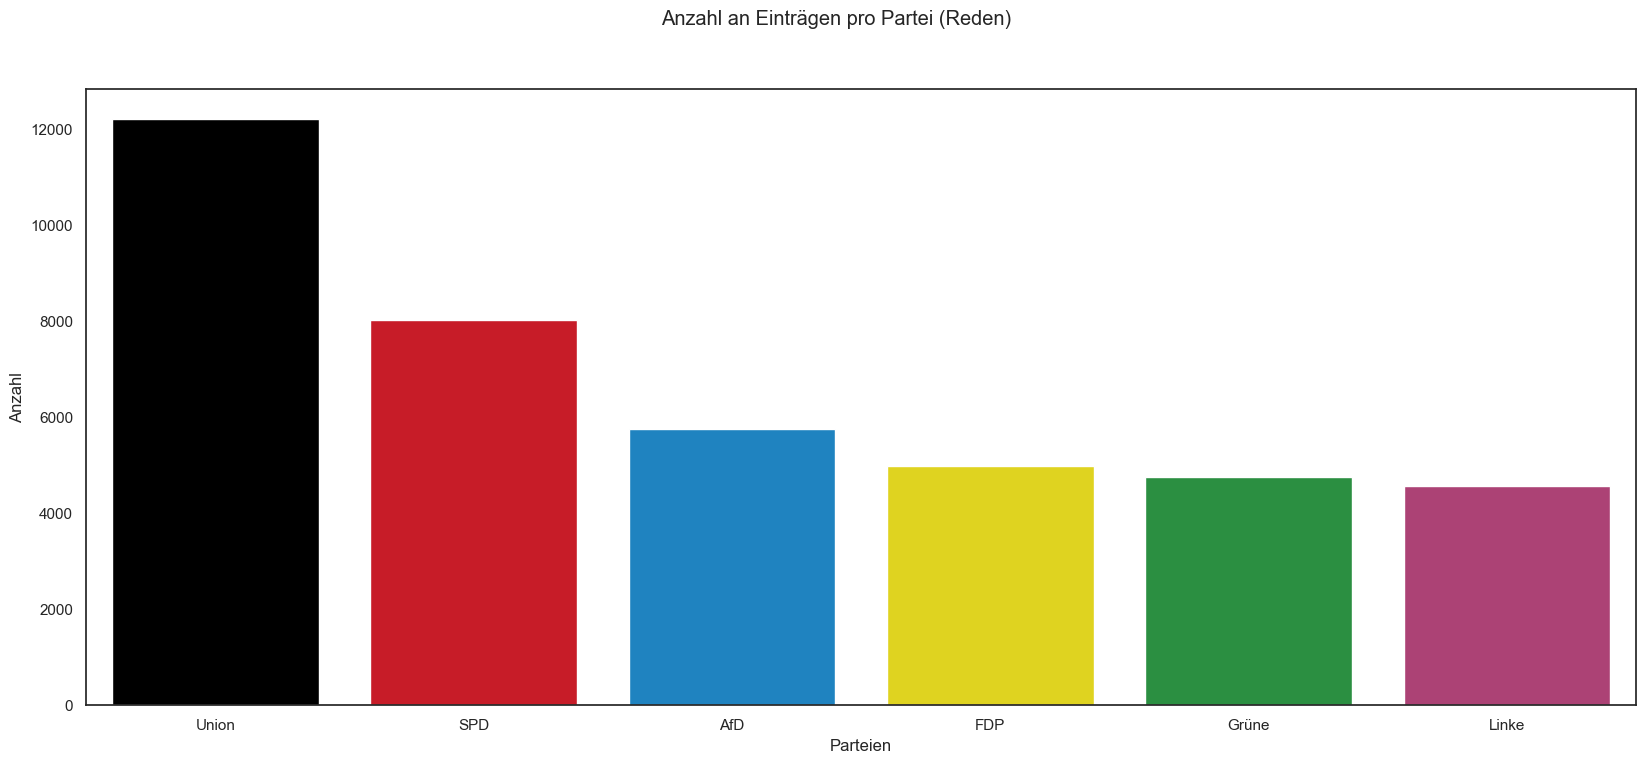
\includegraphics[width=0.9\textwidth]{data/images/speeches_num_samples_after_filter.png}
    \caption{Anzahl an Einträgen für Reden pro Partei nach Bereinigung} \label{fig:speechesNumSamplesAfterFiltering}
\end{figure}

Wie \autoref{fig:speechesNumSamplesAfterFiltering} zu entnehmen ist, stammt mit Abstand der größte Teil der Reden (\num{12200}) von \acp{MdB} der Union, gefolgt von \ac{SPD} (\num{8000}), \ac{AfD} (\num{5800}), \ac{FDP} (\num{5000}), Grünen (\num{4700}) und Linken (\num{4600}). Diese Reihenfolge und Abstufung lässt sich auf das Wahlergebnis der Bundestagswahl \num{2017} (siehe \autoref{subsec:heterogenitätParteien}) und die daraus abgeleitete Sitzverteilung zurückführen, da die Anzahl an gehaltenen Reden von der Größe der jeweiligen Fraktion im Bundestag abhängt.

\begin{figure}[H]
    \centering
    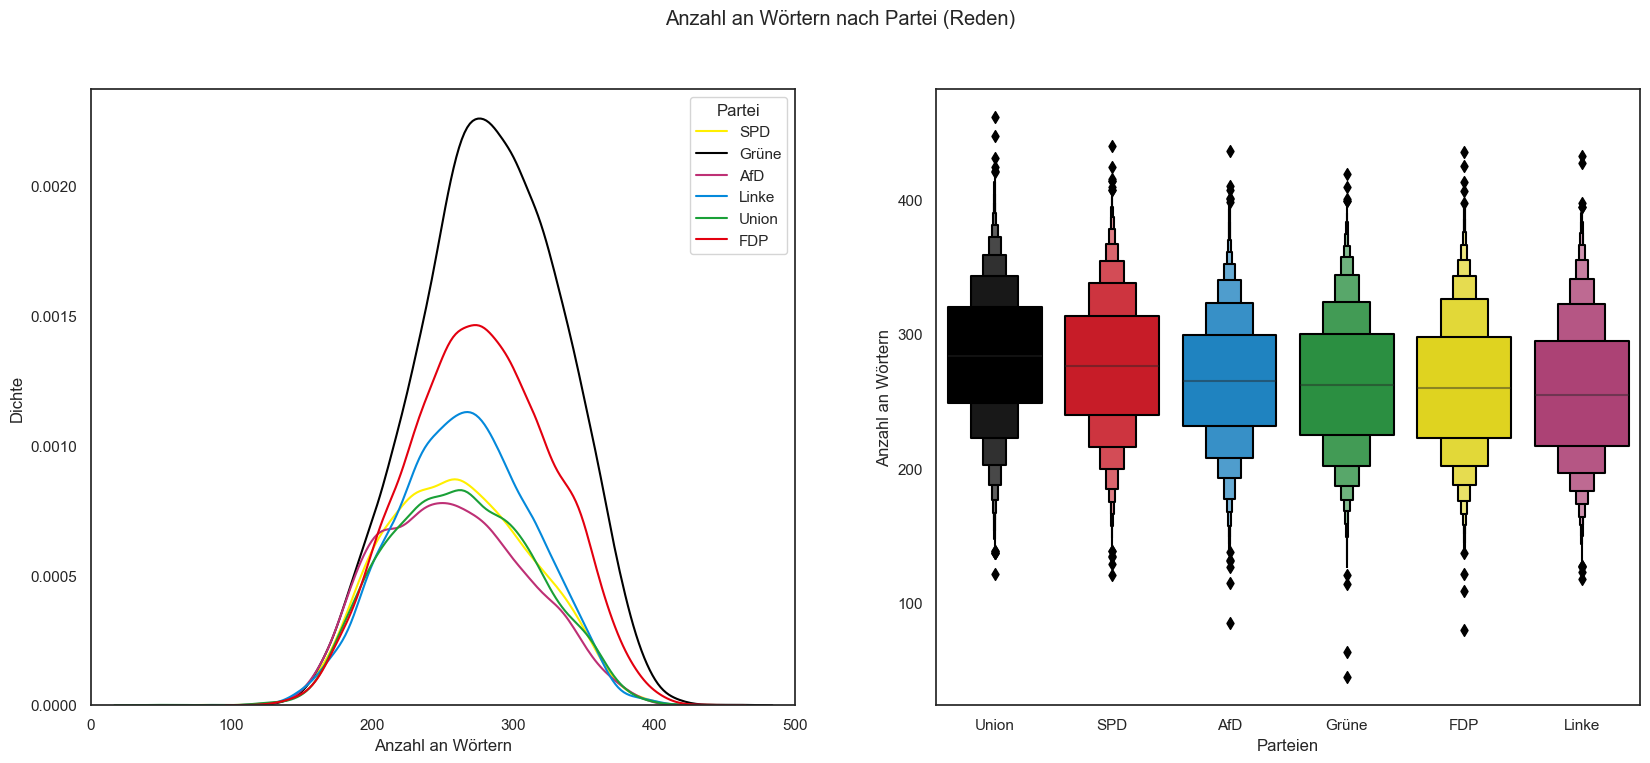
\includegraphics[width=0.9\textwidth]{data/images/speeches_word_count_after_filter.png}
    \caption{Anzahl an Wörtern für Reden nach Bereinigung} \label{fig:speechesWortCountAfterFiltering}
\end{figure}

\autoref{fig:speechesWortCountAfterFiltering} zeigt die Verteilung der Wortanzahl in den Reden pro Partei nach der Bereinigung und der Filterung. Es lässt sich erkennen, dass es im Vergleich zu vor der Bereinigung (siehe \autoref{fig:wordCoundSpeeches}) keine Häufung von Reden unter \num{200} Wörtern mehr gibt.\footnote{Da die Untergrenze von \num{200} Wörtern vor weiteren -- eventuell kürzenden -- Bereinigungsschritten angewandt wird, ist es möglich, dass es weiterhin Reden mit dieser Länge gibt.} Je nach Partei schwankt der Hochpunkt der Verteilung zwischen \num{250} und \num{300} Wörtern. Da zu lange Reden aufgetrennt worden sind, gibt es kaum noch Redetexte über \num{400} Wörtern. Weiterhin sind die Reden der Union im Durchschnitt am längsten. Während die Redetexte der Grünen vor der Bereinigung am kürzesten waren, sind nun die der \ac{FDP} und der Linken kürzer, wenn auch nur marginal.

\begin{figure}[H]
    \centering
    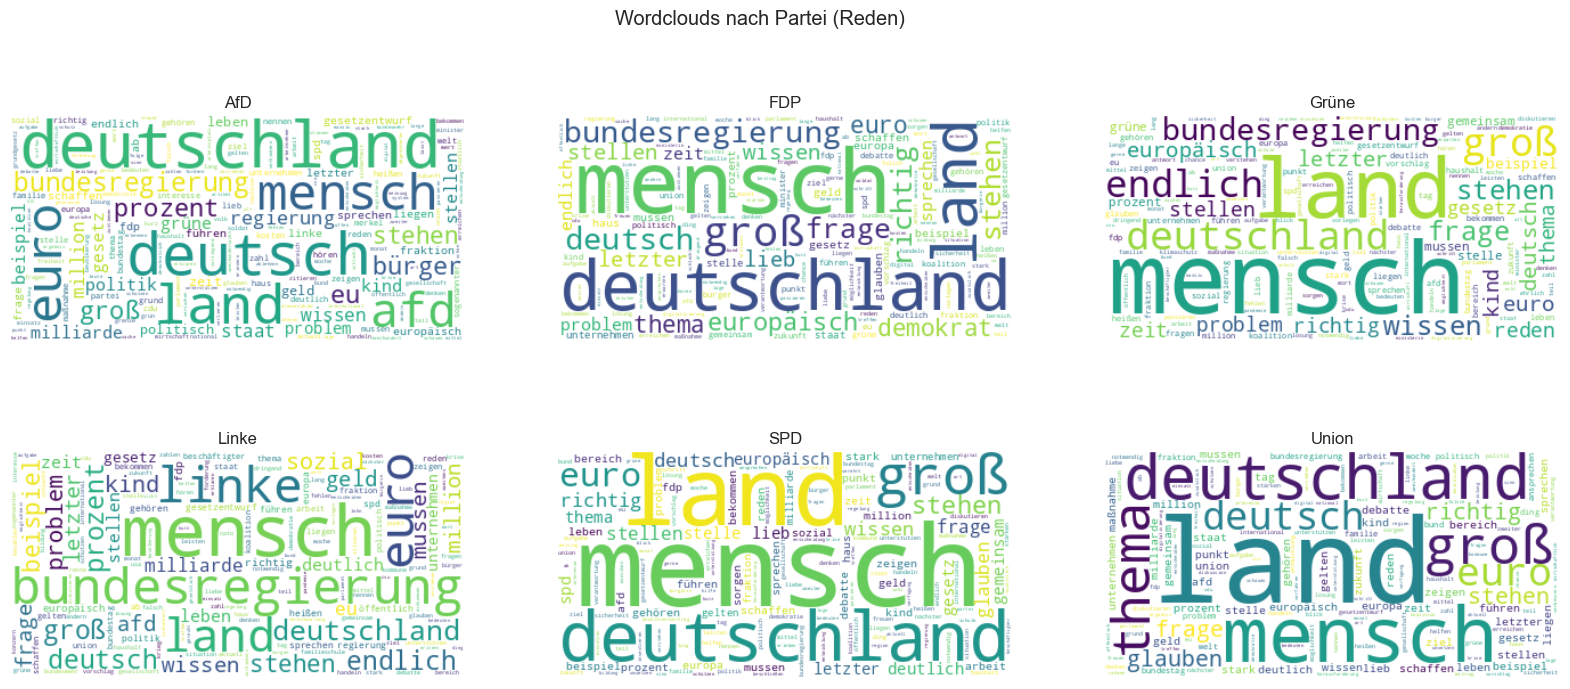
\includegraphics[width=0.9\textwidth]{data/images/speeches_wordclouds.png}
    \caption{Wordclouds mit den meistgenutzten Wörtern in Reden pro Partei} \label{fig:speechesWordclouds}
\end{figure}

Betrachtet man die meistgenutzten Wörter pro Partei, wie in \autoref{fig:speechesWordclouds} mittels Wordclouds dargestellt, fällt auf, dass jede Partei andere Schwerpunkte setzt und dabei ein anderes Vokabular nutzt. Die \ac{AfD} zeigt durch die häufige Nutzung der Wörter \textit{deutsch} und \textit{deutschland} ihren Fokus auf Nationalität, wobei auch bei der \ac{FDP}, \ac{SPD} sowie Union das Wort \textit{deutschland} zahlreich auftritt. Besonders die Oppositionsparteien nutzen das Wort \textit{bundesregierung}, während die Regierungsparteien -- \ac{SPD} und Union -- dieses nur nachrangig verwenden. Daran lässt sich bestätigen, dass die Oppositionsparteien die Bundesregierung in ihren Reden oft direkt adressieren.

\begin{table}[H]
    \centering
    {\footnotesize
    \begin{tblr}{width=\textwidth, hlines, vlines, colspec={l*{3}{Q[si={table-format=1.2},c]}}, row{1}={guard,font=\bfseries,l}} 
        Partei & Negativ & Neutral & Positiv \\
        
        AfD & 0.45 & 0.54 & 0.01 \\
        Grüne & 0.48 & 0.50 & 0.02 \\
        Linke & 0.48 & 0.51 & 0.01 \\
        FDP & 0.41 & 0.57 & 0.02 \\
        SPD & 0.22 & 0.75 & 0.03 \\
        Union & 0.19 & 0.78 & 0.02 \\
    \end{tblr}
    }
    \caption{Prozentuale Sentimentverteilung in Reden pro Partei} \label{tab:sentimentDistributionSpeeches}
\end{table}

Um einen ersten Eindruck über die Ausrichtung der Reden zu bekommen, wurden die Redetexte pro Partei mit einer Sentiment-Analyse untersucht. \autoref{tab:sentimentDistributionSpeeches} zeigt diesbezüglich die Verteilung der Reden mit negativem, neutralem und positivem Sentiment pro Partei. Es lässt sich ein starkes Gefälle zwischen den Regierungsparteien im Untersuchungszeitraum -- SPD und Union -- und den übrigen Oppositionsparteien erkennen: Während der Anteil mit negativem Sentiment bei den Regierungsparteien \SI{22}{\percent} und \SI{19}{\percent} beträgt, liegt dieser bei den Oppositionsparteien mit \SIrange{41}{48}{\percent} deutlich höher. Dies könnte darauf zurückzuführen sein, dass Redner der Oppositionsparteien eher kritisch den Debatten gegenüberstehen, wohingegen Redner der Regierungsparteien hinter ihren Vorschlägen stehen und diese verteidigen.

\subsection*{Wahlprogramme}

Durch die Bereinigung und Filtern hat sich die Anzahl an Datenpunkten nur marginal reduziert. In dem Prozess wurden einige Duplikate entfernt.

\begin{figure}[H]
    \centering
    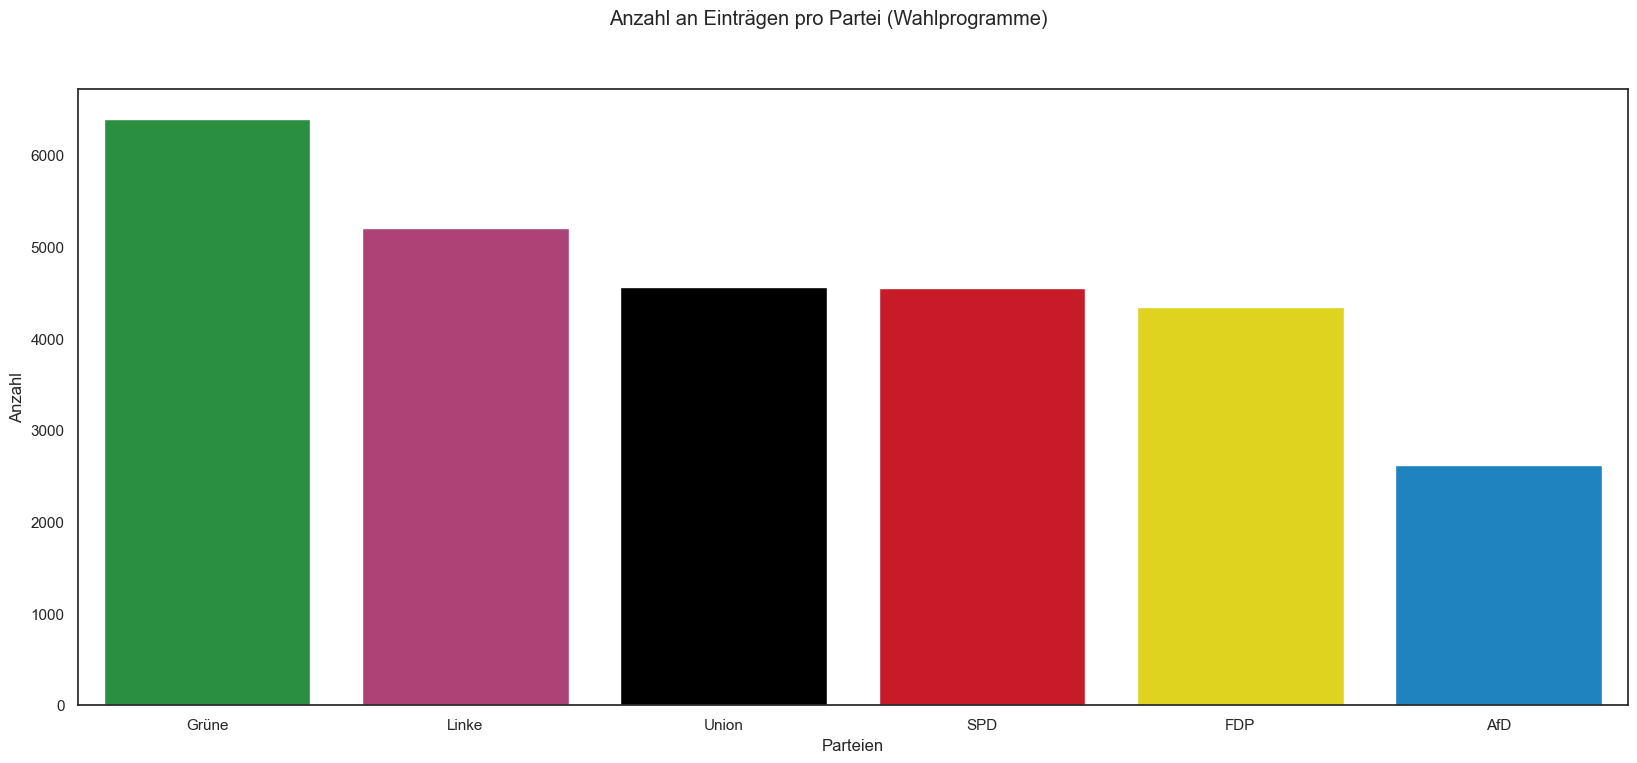
\includegraphics[width=0.9\textwidth]{data/images/party_programs_num_samples_after_filter.png}
    \caption{Anzahl an Einträgen für Wahlprogramme pro Partei nach Bereinigung} \label{fig:partyProgramsNumSamplesAfterFiltering}
\end{figure}

Betrachtet man die Anzahl an Einträgen im Wahlprogramm-Datensatz pro Partei, wie in \autoref{fig:partyProgramsNumSamplesAfterFiltering} dargestellt, lässt sich erkennen, dass von den Grünen mit über \num{6000} am meisten vorliegen, gefolgt von gut \num{5000} von der Linken. Union, \ac{SPD} und \ac{FDP} liegen mit ca. \num{4500} gleich auf. Mit Abstand am wenigsten Absätze -- nämlich \num{2600} -- liegen von der \ac{AfD} vor, da es dort bei sechs Wahlen zu Problemen mit dem Auslesen des Wahlprogramm-Textes aus der \ac{PDF}-Datei gekommen ist.

\begin{figure}[H]
    \centering
    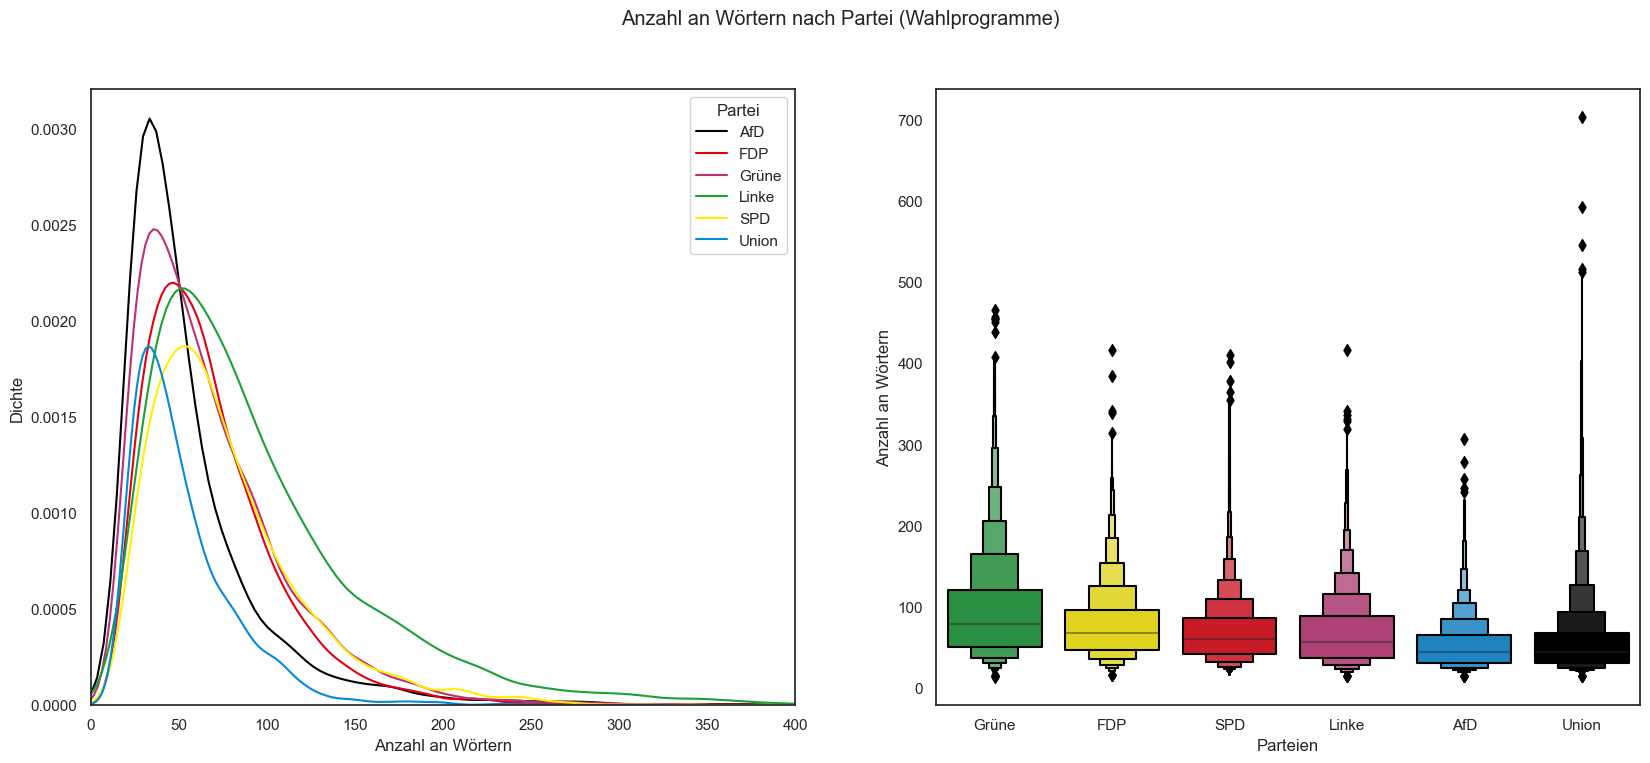
\includegraphics[width=0.9\textwidth]{data/images/party_programs_word_count_after_filter.png}
    \caption{Anzahl an Wörtern für Wahlprogramme nach Bereinigung} \label{fig:partyProgramsWordCountsAfterFiltering}
\end{figure}

\autoref{fig:partyProgramsWordCountsAfterFiltering} zeigt die Verteilung der Wortanzahl in den Wahlprogramm-Absätzen pro Partei nach Bereinigung und Filterung. Es ergeben sich keine grundlegenden Unterschiede im Vergleich zur Verteilung vor der Bereinigung. Weiterhin ist eine Häufung von Reden, die etwa \num{50} Wörter umfassen, festzustellen. Dabei liegen die verschiedenen Parteien etwa gleich auf, mit den längsten Paragraphen bei den Grünen und den kürzesten bei der Union.

\begin{figure}[H]
    \centering
    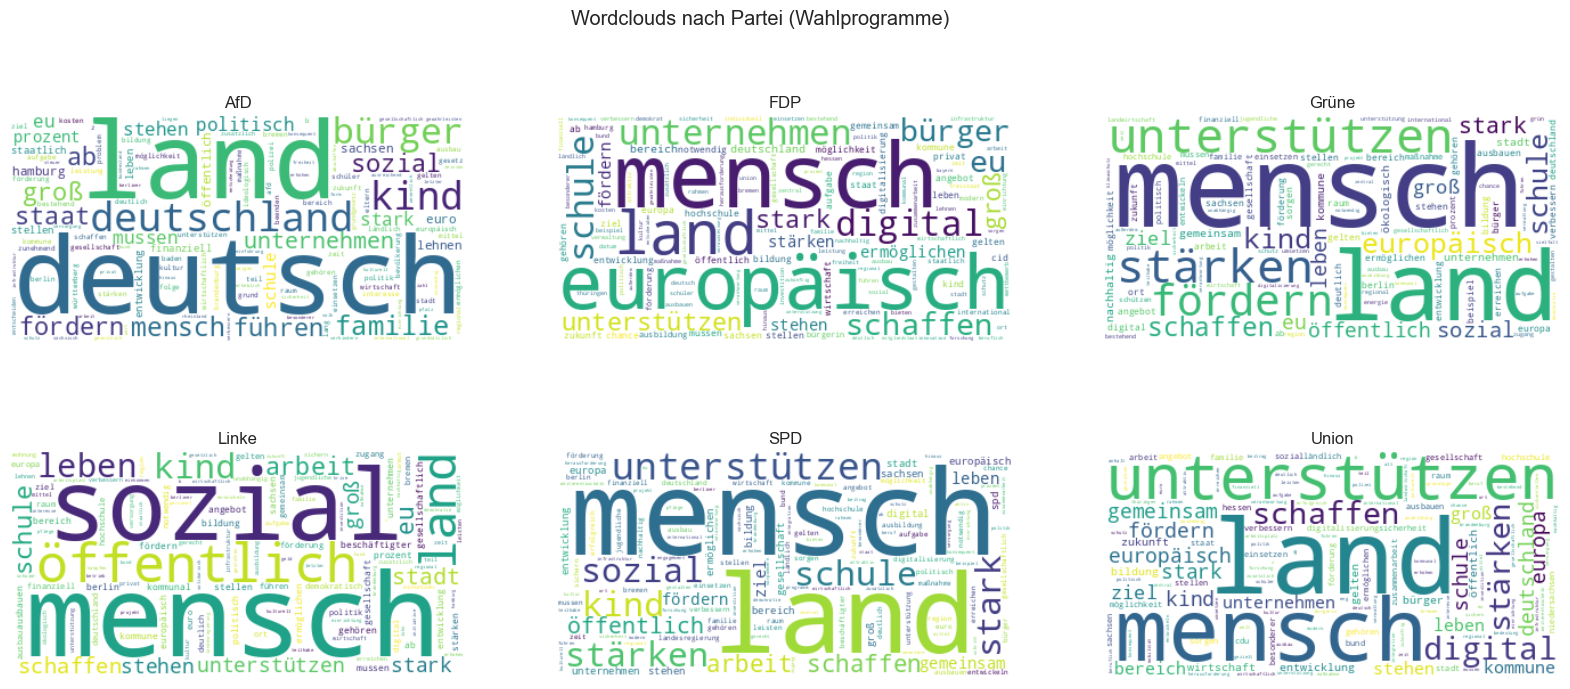
\includegraphics[width=0.9\textwidth]{data/images/party_programs_wordclouds.png}
    \caption{Wordclouds mit den meistgenutzten Wörtern in Wahlprogrammen pro Partei} \label{fig:partyProgramsWordclouds}
\end{figure}

Auch bei den Wahlprogrammen lassen sich einige Erkenntnisse anhand der Wordclouds mit den meist genutzten Wörtern ableiten, die in \autoref{fig:partyProgramsWordclouds} dargestellt sind. Ähnlich wie in den Reden, verwendet die \ac{AfD} je nach Kontext als patriotisch geltende Wörter wie \textit{land}, \textit{deutsch} oder \textit{deutschland}. Anhand viel genutzter Wörter der \ac{FDP} wie \textit{europäisch}, \textit{unternehmen} oder \textit{digital} spiegeln sich Schwerpunkte der Partei wie Wirtschaftsliberalismus und Digitalpolitik sowie eine pro-europäische Haltung wider. Begriffe wie \textit{sozial} und \textit{öffentlich} deuten auf den sozialpolitischen Fokus der Linken hin. Die \ac{SPD} legt einen Fokus auf unter anderem Sozial- und Bildungspolitik (\textit{sozial} sowie \textit{schule}). Grüne und Union nutzen ähnliche Begriffe wie \textit{mensch}, \textit{land} und \textit{unterstützen} am häufigsten. Die Begriffe können je nach Partei unterschiedlich ausgelegt werden.

\begin{table}[H]
    \centering
    {\footnotesize
    \begin{tblr}{width=\textwidth, hlines, vlines, colspec={l*{3}{Q[si={table-format=1.2},c]}}, row{1}={guard,font=\bfseries,l}} 
        Partei & Negativ & Neutral & Positiv \\
        
        AfD & 0.03 & 0.97 & 0.00 \\
        Grüne & 0.03 & 0.96 & 0.01 \\
        Linke & 0.05 & 0.95 & 0.00 \\
        FDP & 0.02 & 0.97 & 0.01 \\
        SPD & 0.01 & 0.98 & 0.01 \\
        Union & 0.01 & 0.98 & 0.01 \\
    \end{tblr}
    }
    \caption{Prozentuale Sentimentverteilung in Wahlprogrammen pro Partei} \label{tab:sentimentDistributionPartyPrograms}
\end{table}

Die Auswertung des Sentiments in den Wahlprogramm-Texten des Datensatzes, die in \autoref{tab:sentimentDistributionPartyPrograms} gezeigt ist, ergibt, dass die Wahlprogramme primär in neutraler Stimmung formuliert sind (bei jeder Partei mindestens \SI{95}{\percent}). Die größte Abweichung davon zeigt die Linke, deren Wahlprogramme zu einem Anteil von \SI{5}{\percent} als negativ kategorisiert werden. Diese Betrachtungen lassen sich anhand der Natur von Wahlprogrammen erklären. Diese verfolgen das Ziel neutral über geplante politische Vorhaben zu informieren, während Reden und Tweets auch emotionale und subjektive Aussagen enthalten. Daher erklärt sich der geringe Anteil an Textabschnitten, denen eine negative oder positive Gesinnung attestiert wird.

\section{Modeling} \label{sec:modeling}

% TODO: Review and add ideas for modeling

\begin{itemize}
    \item Datenquellen erst einzeln trainieren
    \item Datenquellen in verschiedenen Kombinationen trainieren
    \item Undersampling nach Partei 
\end{itemize}

\subsection{Feature Engineering} \label{subsec:featureEngineering}

% TODO: This are only ideas and options for additional features 
% TODO: Evaluate the features

\subsubsection{Sentiment}

Eine Limitation von den herkömmlichen \ac{ML} Modellen ist die Klassifikation von Polysemie \autocite[48\psq]{kowsari_text_2019}. 

% TODO: Find source

Ein Ansatz, um diese Limitation zu mindern, ist es, den Sentiment eines Textes zu berechnen. Ziel dieser Technik ist es nicht nur festzustellen, ob sich ein Politiker zum Beispiel zur \ac{AfD} äußert oder nicht, sondern ebenfalls, ob seine Äußerungen positiv, neutral oder negativ sind.

% TODO: Add timeline for ML Models

Die einfachste Methode, um den Sentiment von deutschen Texten zu ermitteln, sind Sentiment-Wörterbücher wie \textit{SentiWS}, \textit{BAWL-R} und \textit{GermanPolarityClues} \autocite[1627\psq]{guhr_training_2020}. CNN, SVM, Bi-LSTM, \dots

Die bisherigen regelbasierten Ansätze, als auch \ac{ML} Modelle wie \acp{SVM}, \acp{CNN} und \acp{LSTM} erreichen einen F1-Score von bis zu \num{74.9}. Alternativ zu diesen Ansätzen stellen \textcite{guhr_training_2020} ein \ac{BERT}-basiertes \ac{ML} Modell bereit. Dieses wurde mittels der folgenden Datensätze trainiert: \textit{PotTS}, \textit{SB10k}, \textit{GermEval-2017}, \textit{Scare}, \textit{Filmstarts}, \textit{holidaycheck}, \textit{leipzig-wikipedia} und \textit{Emotions}. Das Modell erreicht einen F1-Score von \num{0.9636} und ist somit den vorherigen Modellen deutlich überlegen \autocite[1631]{guhr_training_2020}.

\subsubsection{Gendern}

- Verhältnis Wörter/Gendersterne oder True/False
- Check mit RegEx ob gegendert wird und setze variable

\subsubsection{Dokumenttyp}

- Tweet, Speech, \dots

\subsection{Baseline Models}

% TODO: Update scores

\begin{table}[H]
    \centering
    {\footnotesize
    \begin{tblr}{width=\textwidth, hlines, vlines}
        \textbf{Modell} & \textbf{Datensatz} & \textbf{Precision} & \textbf{Recall} & \textbf{\(F_1\) Score} \\ 

        \textbf{SVM + \acs{BoW}} & Tweets & \num{0.59} & \num{0.59} & \num{0.59} \\
        \textbf{SVM + \acs{BoW}} & Wahlpro\-gramme & \num{0} & \num{0} & \num{0} \\
        \textbf{SVM + \acs{BoW}} & Reden & \num{0} & \num{0} & \num{0} \\

        \textbf{Kombiniert} & \textbf{\num{0}} & \textbf{\num{0}} & \textbf{\num{0}} \\
    \end{tblr}
    }
    \caption{Scores für Baseline Modelle auf Basis von \ac{BoW} und \ac{TF-IDF}} \label{tab:overviewScoresBaseline}
\end{table}

\subsection{Advanced Models}

\subsubsection{FastText}

% TODO: Update and add plots for other datasets

\begin{figure}[H]
    \begin{subfigure}{.5\textwidth}
      \centering
      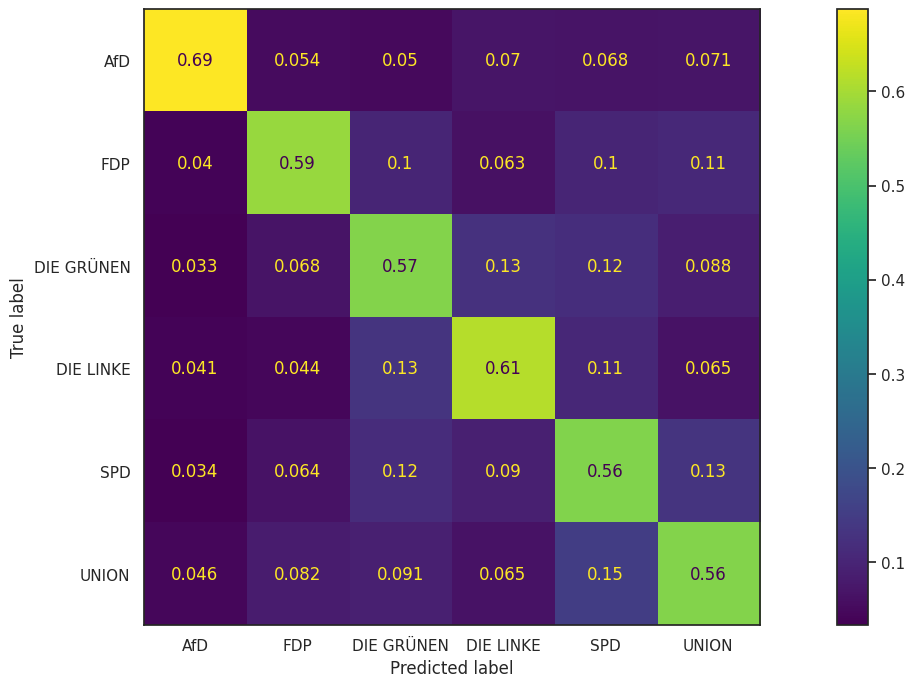
\includegraphics[width=0.9\linewidth]{data/images/fasttext_tweets_confusion.png}
      \caption{Tweets von \acs{MdB}} \label{sfig:confusionMatrixFastTextTweets}
    \end{subfigure}
    \begin{subfigure}{.5\textwidth}
      \centering
      \missingfigure{Wahlprogramme}
      \caption{Wahlprogramme} \label{sfig:confusionMatrixFastTextManifest}
    \end{subfigure}
    \begin{subfigure}{.5\textwidth}
      \centering
      \missingfigure{Reden}
      \caption{Reden im Deutschen Bundestag} \label{sfig:confusionMatrixFastTextSpeeches}
    \end{subfigure}
    \begin{subfigure}{.5\textwidth}
      \centering
      \missingfigure{Kombiniert}
      \caption{Kombinierten Datensatz} \label{sfig:confusionMatrixFastTextAll}
    \end{subfigure}
    \caption{Konfusion Matritzen für \texttt{fasttext}} \label{fig:confusionMatrixFastText}
\end{figure}

\begin{itemize}
    \item Parteien, welche politisch näher beieinander liegen, lassen sich schlechter Klassifizieren
\end{itemize}

% TODO: Update scores

\begin{table}[H]
    \centering
    {\footnotesize
    \begin{tblr}{width=\textwidth, hlines, vlines, colspec={l*{3}{Q[si={table-format=1.2},c]}}, row{1}={guard,font=\bfseries,l}, row{5}={font=\bfseries}}
        Datensatz & Precision & Recall & \(F_1\) Score \\ 

        Tweets & 0.59 & 0.59 & 0.59 \\
        Wahlpro\-gramme & 0 & 0 & 0 \\
        Reden & 0 & 0 & 0 \\

        Kombiniert & 0 & 0 & 0 \\
    \end{tblr}
    }
    \caption{Scores für Supervised Learning mittels \texttt{fasttext} (\texttt{weighted avg})} \label{tab:overviewScoresFastText}
\end{table}

\subsubsection{BERT}

Lorem Ipsum

\subsubsection{ELMo}

Lorem Ipsum

\subsection{Limitationen}

\subsubsection{Feature Engineering}

% TODO: Add example for polysemy

Durch Methoden wie \ac{BoW} und \ac{TF-IDF} gehen syntaktische, als auch semantische Zusammenhänge verloren \autocite[48\psq]{kowsari_text_2019}. Dies führt dazu, dass Modelle wie \ac{SVM} und Random Forest ausschließlich die verwendeten Wörter und deren Anzahl in Betracht zieht, aber nicht die tiefere Bedeutung im Kontext des Satzes. Nach \textcite{kowsari_text_2019} versuchen Modelle wie Word2Vec, GloVe und \texttt{fasttext} zumindest syntaktische und semantische Zusammenhänge zu berücksichtigen, jedoch haben selbst diese Modelle Schwierigkeiten, Polysemie\footnote{Sätze mit mehreren Bedeutungen} zu klassifizieren.

\subsubsection{Sprache}

% TODO: Add sources and examples

Des Weiteren ergibt sich aus der Wahl der Datenquellen (Wahlprogramme, Reden und Tweets) eine Annahme/Voraussetzung/Bias geben über der verwendeten Sprache. Wahlprogramme, Reden und Tweets von Politikern weisen zwar parteispezifische Wörter auf, jedoch ist die semantische und syntaktische Komplexität der Sätze überdurchschnittlich hoch. Ebenfalls ist die Menge an Rechtschreibfehlern und verwendetem Slang geringer als bei anderen Textarten. Daraus folgt, dass die Performance der trainierten Modelle voraussichtlich signifikant schlechter ist, wenn Texte sprachlich (semantisch und syntaktisch) stark von den Trainingsdaten abweichen.

\subsubsection{Politische Nähe}

% TODO: Add sources and image
% TODO: Reason --> Politisches Viereck (links -- rechts, ...)

Parteien, welche ähnliche politische Ideale verfolgen, identische Themenschwerpunkte haben, lassen sich schlechter klassifizieren.

\section{Fazit} \label{sec:crispConclusion}

\begin{itemize}
    \item Gendern inkompatibel mit Lemmatizing und daher problematisch
\end{itemize}
